\input templates/header
\title[DS - Rollback-Recovery]{\textbf{Distributed Algorithms}\\Rollback-Recovery}

\graphicspath{{figs/15/}}

\newcommand{\Textbullet}{{\tiny \textbullet \quad}}

\begin{document}

%-------------------------------------------------------------------------
\FrameTitle{}


\section{Introduction}

\begin{frame}{Reliability -- different techniques, different focus}
	
\begin{block}{Fault tolerance}
Offers the abstraction of a reliable system that tolerates faults
\BI
\item \alert{Group communication}\\
 Offers an abstraction of an ideal communication system that simplifies the development of reliable applications
\EI
\end{block}
\begin{block}{Fault-recovery}
Once a fault occurs, we want to recover to a previous correct state
\BI
\item \alert{Transactions}\\
  Data-oriented application	
\item \alert{Rollback-recovery}\\
Long-running applications such as scientific computing, where failures are rare but process state is important
\EI 
\end{block}
\end{frame}


\begin{frame}{The idea}
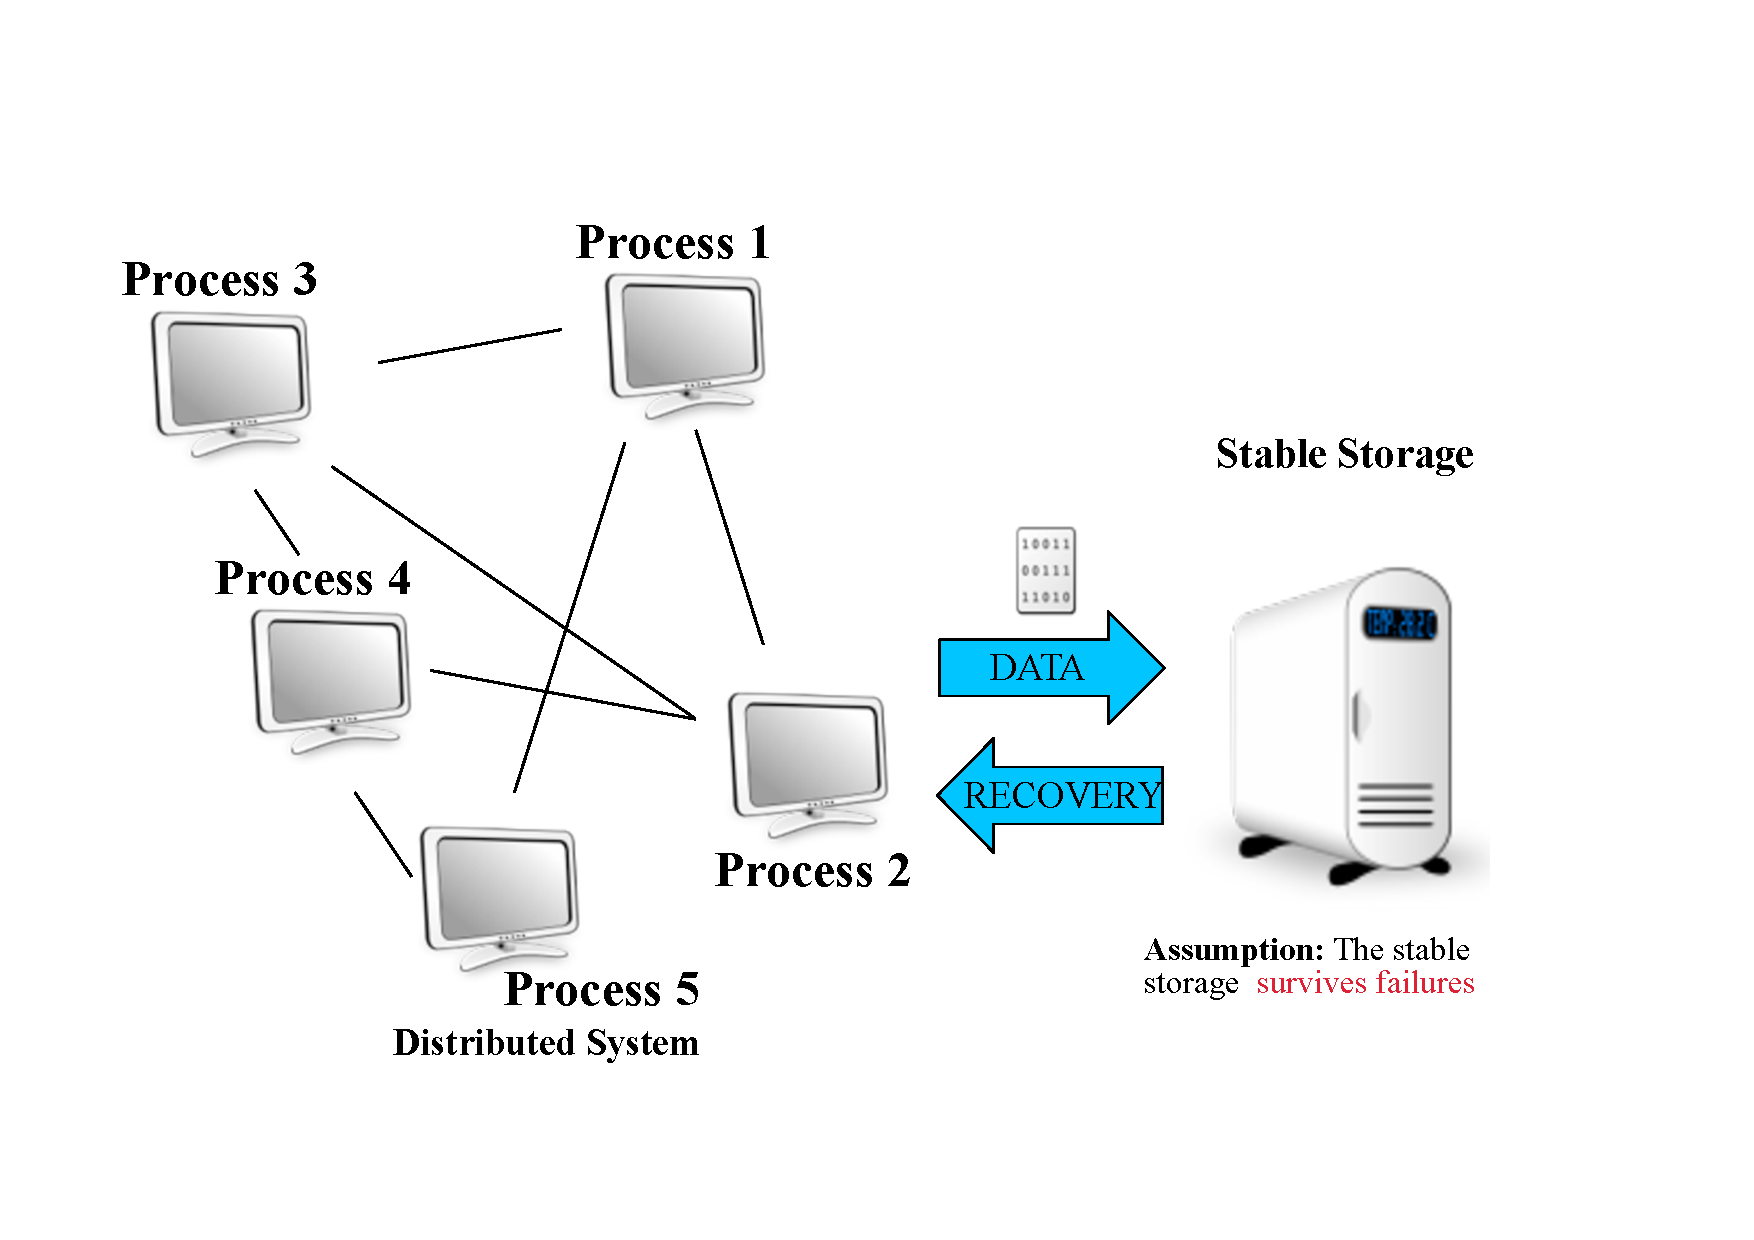
\includegraphics[width=\textwidth]{rr-idea}
\end{frame}

\begin{frame}{The idea}
	
\BIL
\item \alert{Processes}:
\BI
\item have access to a stable storage that survives all tolerated failures 
\item disks, RAID arrays
\EI
\item \alert{Stable storage}:
\BI
\item is used to save recovery information periodically during failure-free periods.
\EI
\item \alert{Upon a failure}:
\BI
\item a failed process uses the saved information to restart the computation from an intermediate state, thereby reducing the amount of lost computation
\EI
\EIL
\end{frame}

\section{Background and definition}

\subsection{System model}

\begin{frame}{System model}

\begin{block}{Processes}
\BI
\item Fixed number $N$ of processes 
\item Process failures
\BI
\item Fail-stop model
\item Volatile memory is lost
\item Access to stable storage that survives failures
\EI
\EI
\end{block}
\begin{block}{Communication}
\BI
\item No partitioning
\item Different models:
 \BI 
  \item Unreliable channels (lose, duplicate, reorder) 
  \item Reliable channels (FIFO)
 \EI
\item Different protocols for different models
\EI
\end{block}
\end{frame}

\begin{frame}{System model}
\begin{block}{Determinism vs non-determinism}
\BIL
\item State-intervals, each started by a non-deterministic event
\item Execution during each state interval is deterministic
\item \alert{PieceWise Deterministic} assumption (PWD)\\
\emph{
It is possible to capture sufficient information about non-deterministic events that initiate the state intervals
}
\EIL
\end{block}
\begin{figure}
	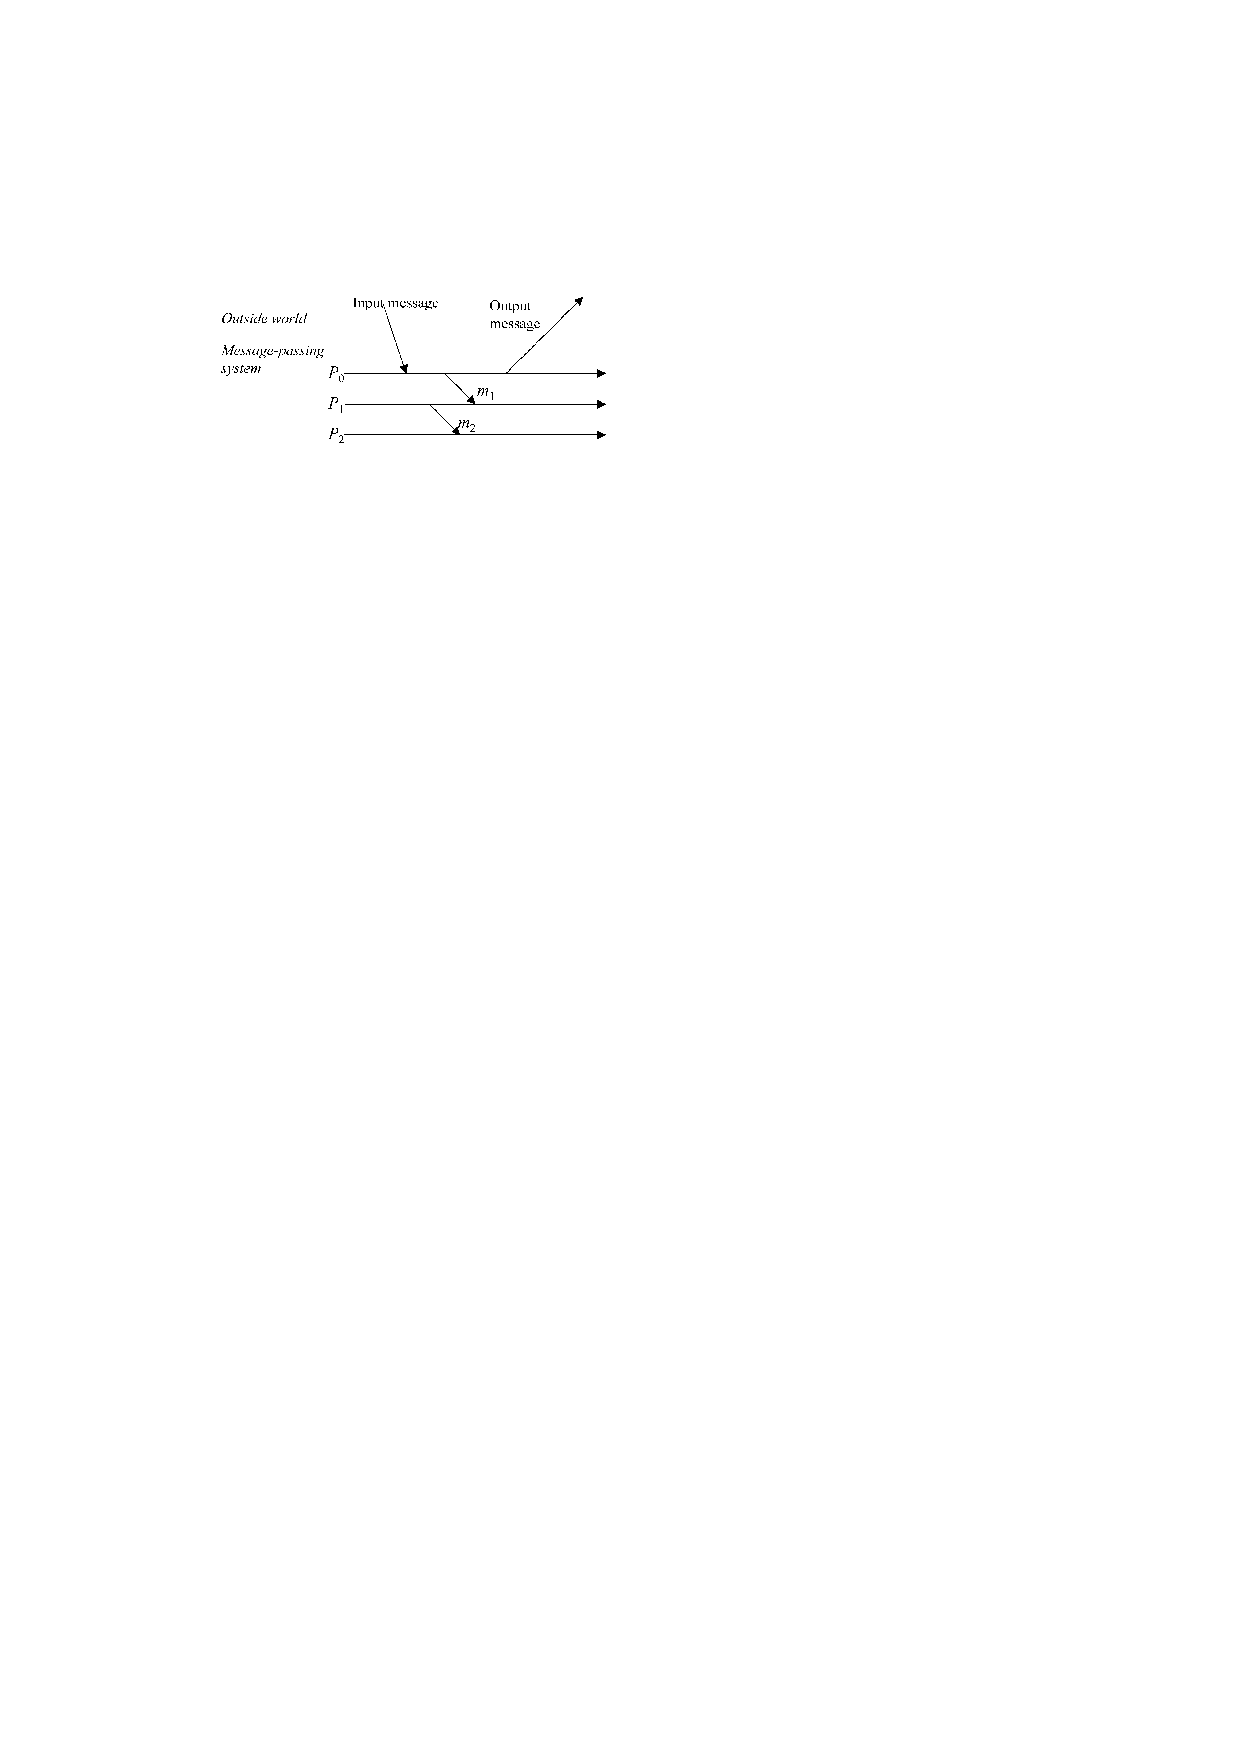
\includegraphics[width=0.6\textwidth]{system}
\end{figure}	

\end{frame}

\subsection{Saving state}


\begin{frame}{Correctness condition}
\begin{block}{Correctness}
A system recovers correctly if its internal state after the recovery is consistent with the observable behavior of the system before the failure.
\end{block}
\bigskip
\BI
\item Rollback-recovery protocols therefore must persist information
\BI
\item about the internal interactions among processes 
\item the external interactions with the outside world
\EI
\EI
\end{frame}

\begin{frame}{Basic approaches}
	
\begin{block}{Checkpointing}
\BI
\item Store the states of the participating processes, called checkpoints 
\EI
\end{block}
\begin{block}{Message/event logging}
\BI
\item Log messages exchanged among the processes 
\item Log interactions with input and output devices
\item In general, log events that occur at each process	
\EI
\end{block}	
\end{frame}

\begin{frame}{An hybrid approach}
\BIL
\item \alert{When executing}
\BI
\item Make a periodic "big" checkpoint
\item More frequently, make incremental additions
\EI
\item \alert{When recovering}
\BI
\item Restore latest checkpoint
\item Replay messages/events stored in logs
\item Combining checkpoints with message logging makes it possible to restore a state that lies beyond the most recent checkpoint
\EI
\EIL
\end{frame}

\begin{frame}{How to save the state -- ask the application}
	
\BIL
\item \emph{A checkpoint should include data that can't be regenerated
in a quick, straightforward way}
\item Some applications might have massive data structures while they run
\BI
\item ... some of them may have been read from the disk at startup
\item ... some of them may rarely be changed
\item ... some of them may have been generated on the fly
\EI
\item Example: scientific computing
\EIL
\end{frame}

\begin{frame}{How to save the state -- transparently}
\BIL
	\item  \emph{A checkpoint should include the entire state of a process/system}
		\BI
		\item Write out its memory "layout"
		\item Contents of all pages
		\item Contents of registers
		\EI
	\item Resume the process by simply reloading its entire state
		\BI
		\item Windows XP, GNU/Linux OSs do this for "hibernate" feature
		\item Virtual machines
		\EI
	\item Potentially, very fast
\EIL
\end{frame}

\begin{frame}{How to save the state}
\BIL
	\item How (not) to take a checkpoint
		\BI
		\item Block execution, save entire process state to stable storage
		\item Very high overhead during failure-free execution
		\item Lots of unnecessary data saved on stable storage
		\EI
	\item How to take a checkpoint
	\BI
		\item Take checkpoints incrementally
			\BI
			\item Save only pages modified since last checkpoint
			\item Use "dirty" bit to determine which pages to save
			\EI
		\item Save only "interesting" parts of address space
			\BI
			\item Use application hints or compiler help to avoid saving useless data (e.g. dead variables)
			\EI
		\item Do not block application execution during recovery
			\BI
			\item Copy-on-write	
			\EI
	\EI
\EIL	
\end{frame}

\begin{frame}{How to save state}
\BIL
\item Problem: a program with a bug can...
\begin{enumerate}
\item Crash due to a corrupt data structure
\item Roll back until the last checkpoint
\item Reload the same (still corrupt) structure
\item ... goto 1
\end{enumerate}
\item "Rebuilding" data structures from scratch avoid this risk
\EIL
\end{frame}

\subsection{Stable storage}

\begin{frame}{Stable storage}
	
\BIL
\item Do not confuse it with the disk storage (frequently) used to implement it.
\item Abstraction
\BI
\item Recovery data must persist through the tolerated failures and the their corresponding recoveries
\EI
\item Implementations
	\BI
	\item Tolerating a single failure
		\BI
		\item Volatile memory of another process
		\EI
	\item Tolerating transient failures
		\BI
		\item Local disk at each host
		\EI
	\item Tolerating non-transient failures
		\BI
		\item Persistent medium outside the host on which a process is running
		\EI
	\EI
\EIL
\end{frame}

\begin{frame}{Consistent global checkpoint}

\begin{columns}
\begin{column}{0.48\textwidth}
\begin{block}{\alert{Local checkpoint}}
A snapshot of a local state of a process
\end{block}
\end{column}
\begin{column}{0.48\textwidth}
\begin{block}{\alert{Global checkpoint}}
A set of local checkpoints, one from each process
\end{block}
\end{column}
\end{columns}

\begin{block}{\alert{Consistent global checkpoint}}
A global checkpoint such that no message is sent by a process after taking its
local checkpoint, that is received by another process before taking its local
checkpoint
\end{block}
\begin{figure}
	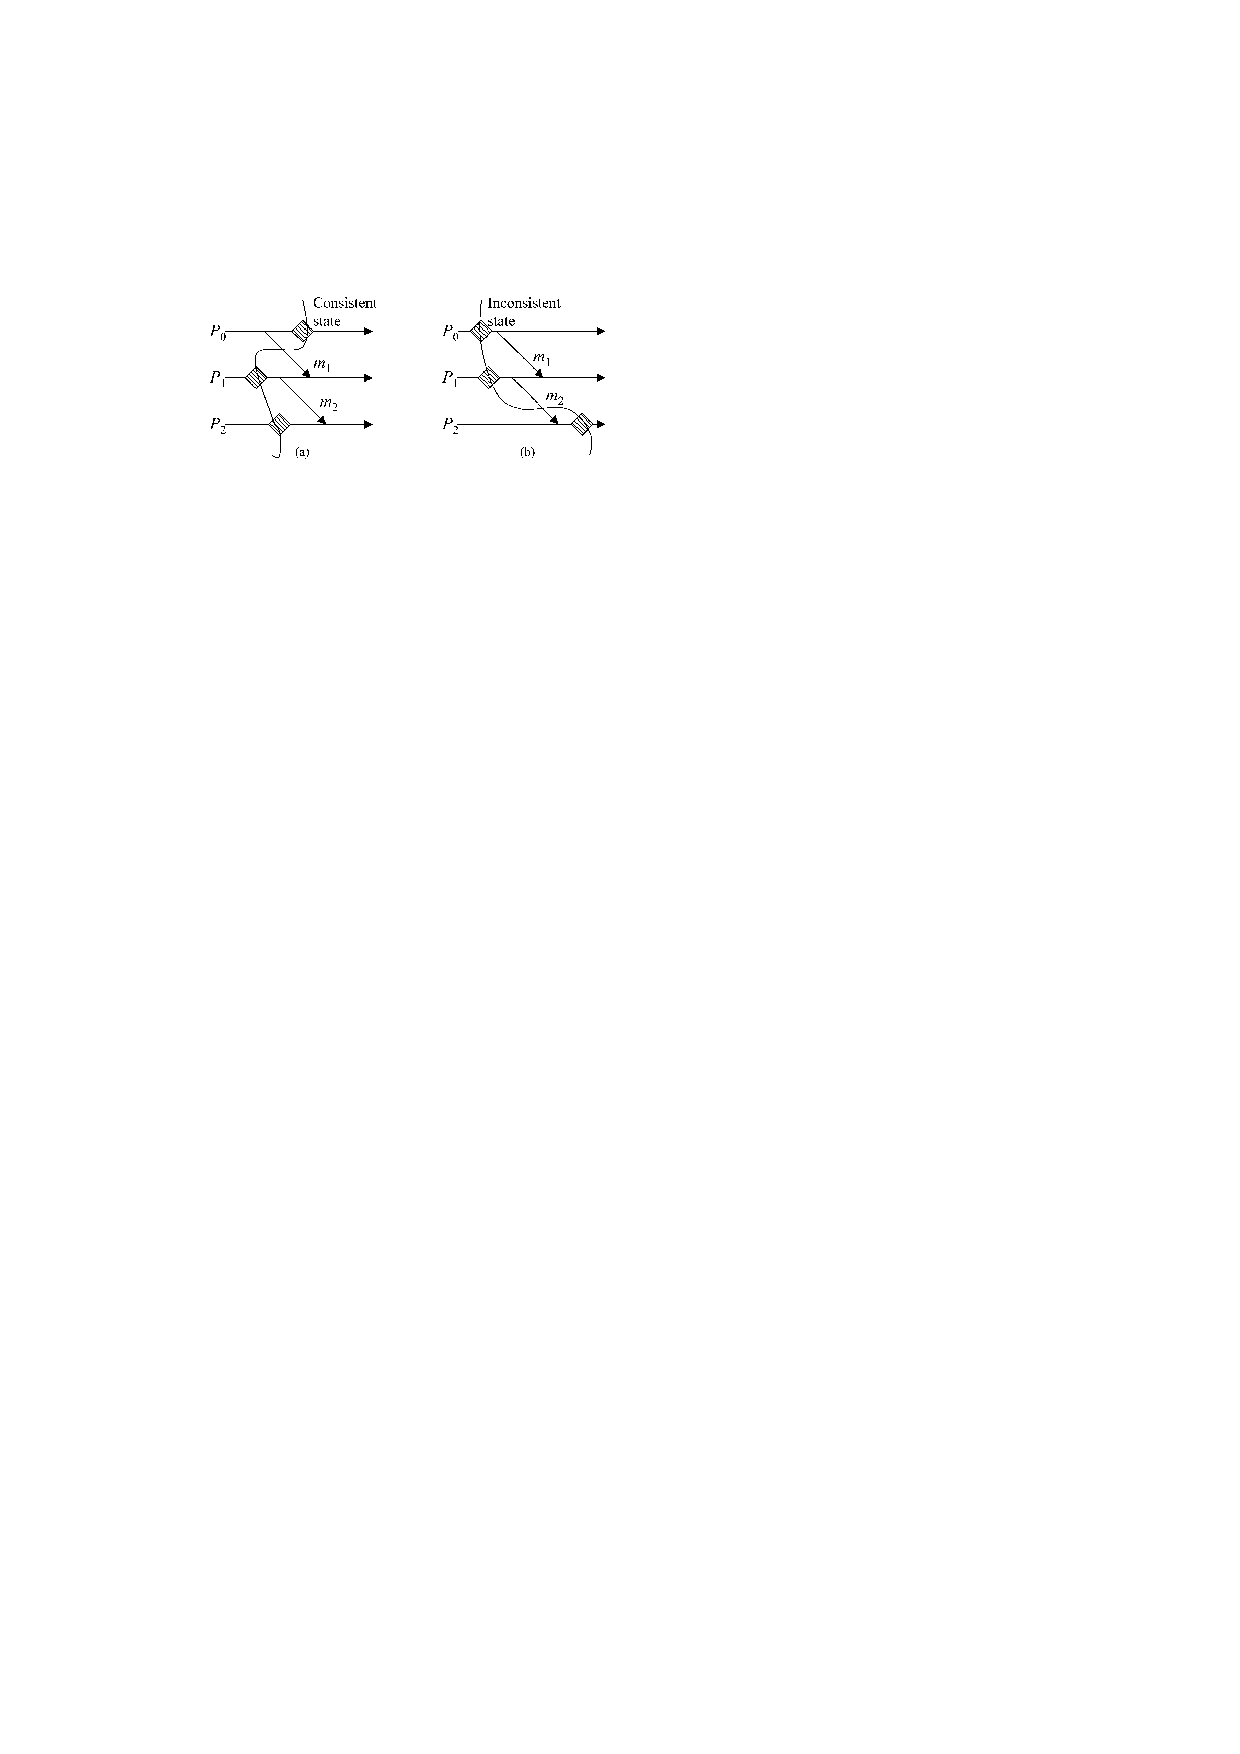
\includegraphics[width=0.5\textwidth]{consistent}
\end{figure}
\end{frame}

\begin{frame}{Type of messages}

\begin{overprint}
\onslide<1-2|handout:1-2>
\begin{block}{\alert{In-transit messages}}
\BI
\item Messages sent, not yet received before recovery line
\item No problem with global state consistency
\item Can be lost or delayed
\EI
\end{block}
\onslide<3-4|handout:3-4>
\begin{block}{\alert{Lost messages}}
\BI
\item Send not undone, receive undone
\item Lost messages must be replayed
\item If implemented over
	\BI 
	\item unreliable communication, application is responsible
	\item reliable communication, recovery algorithm is responsible
	\EI
\EI
\end{block}
\onslide<5-6|handout:5-6>
\begin{block}{\alert{Delayed messages}}
\BI
\item Messages whose receive is not recorded because the receiving process was
either down or the message arrived after the rollback of the receiving process
\EI
\end{block}
\onslide<7|handout:7>
\begin{block}{\alert{Orphan messages}}
\BI
\item Send undone, receive not undone
\item To be avoided if we want consistent global states
\item No examples here
\EI
\end{block}
\onslide<8|handout:8>
\begin{block}{\alert{Duplicate messages}}
\BI
\item Duplicate messages arise due to message logging and replaying during process recovery
\item Example: $m_5$ will be replayed, so it can arrive twice at $P_3$
\EI
\end{block}
\end{overprint}

\begin{overprint}
\onslide<1|handout:1>
\begin{figure}
	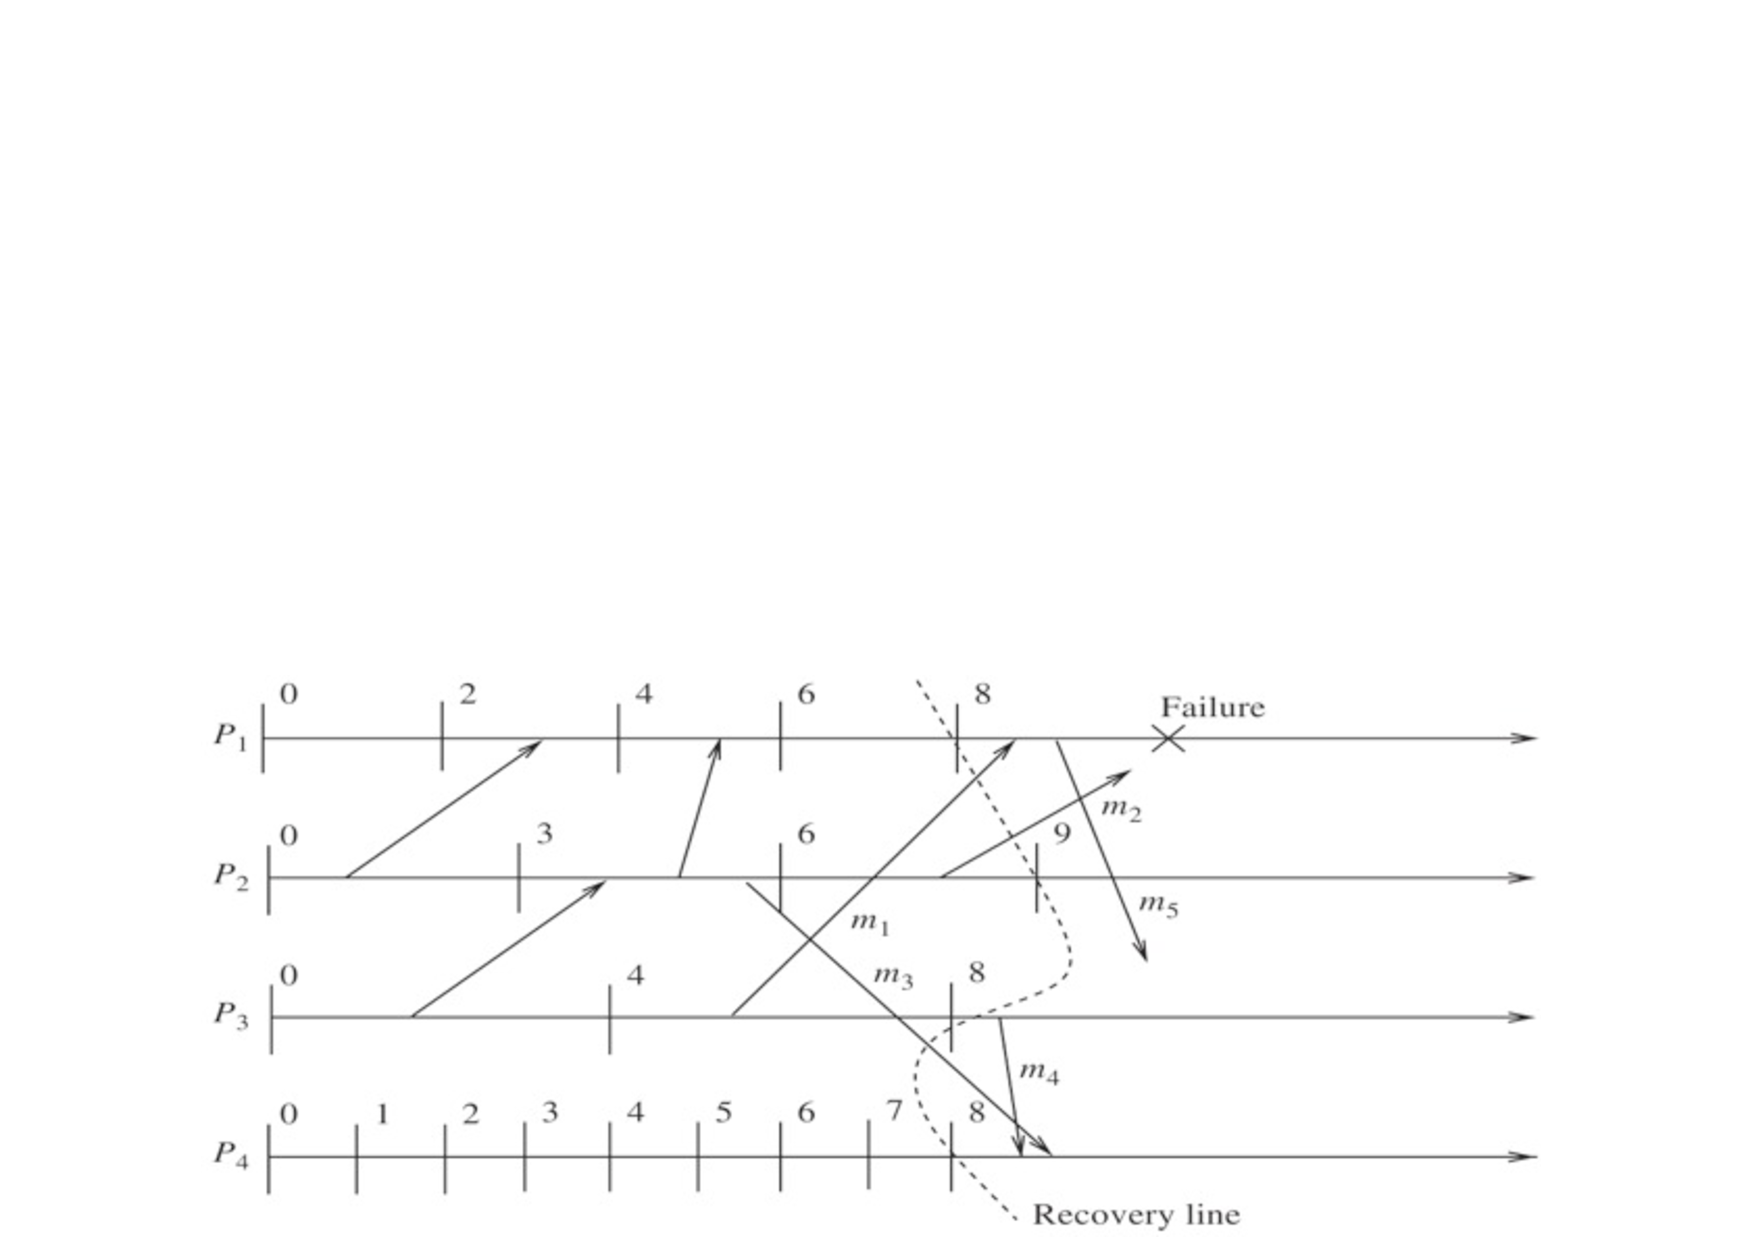
\includegraphics[width=0.7\textwidth,page=1]{messages}
\end{figure}
\onslide<2|handout:2>
\begin{figure}
	\includegraphics[width=0.7\textwidth,page=2]{messages}
\end{figure}
\onslide<3|handout:3>
\begin{figure}
	\includegraphics[width=0.7\textwidth,page=3]{messages}
\end{figure}
\onslide<4|handout:4>
\begin{figure}
	\includegraphics[width=0.7\textwidth,page=4]{messages}
\end{figure}
\onslide<5|handout:5>
\begin{figure}
	\includegraphics[width=0.7\textwidth,page=5]{messages}
\end{figure}
\onslide<6|handout:6>
\begin{figure}
	\includegraphics[width=0.7\textwidth,page=6]{messages}
\end{figure}
\onslide<7|handout:7>
\begin{figure}
	\includegraphics[width=0.7\textwidth,page=7]{messages}
\end{figure}
\onslide<8|handout:8>
\begin{figure}
	\includegraphics[width=0.7\textwidth,page=7]{messages}
\end{figure}
\end{overprint}
\end{frame}

%-------------------------------------------------------------------------
\begin{frame}{Interaction with outside world}

\BI
\item The outside world cannot be "rolled back"
	\BI
	\item A printer cannot "unprint"
	\item A bancomat cannot ask money back \ldots
	\EI
\item Special "Outside World Process" (OWP)
	\BI
	\item Cannot fail
	\item Cannot maintain state, cannot participate in the recovery protocol
	\EI
\item Input
	\BI
	\item Input cannot be replayed by OWP, should be replayed by R-R
	\item External messages must be logged
	\EI
\EI

\end{frame}

%-------------------------------------------------------------------------
\begin{frame}{Interaction with the outside world}
\BI
\item Output commit problem
\BI
\item The externally visible behavior of a rollback-recovery system must be equivalent to some failure-free execution
\item Equivalent $\equiv$ same messages to OWP, same order
\EI
\item How to do it
\BI
\item Commit a message to the outside world as soon is determined that the state that generated the message will never need to be rolled back
\EI
\EI
\end{frame}

%-------------------------------------------------------------------------
\begin{frame}{Output commit problem}

\begin{overprint}
\onslide<1|handout:1>
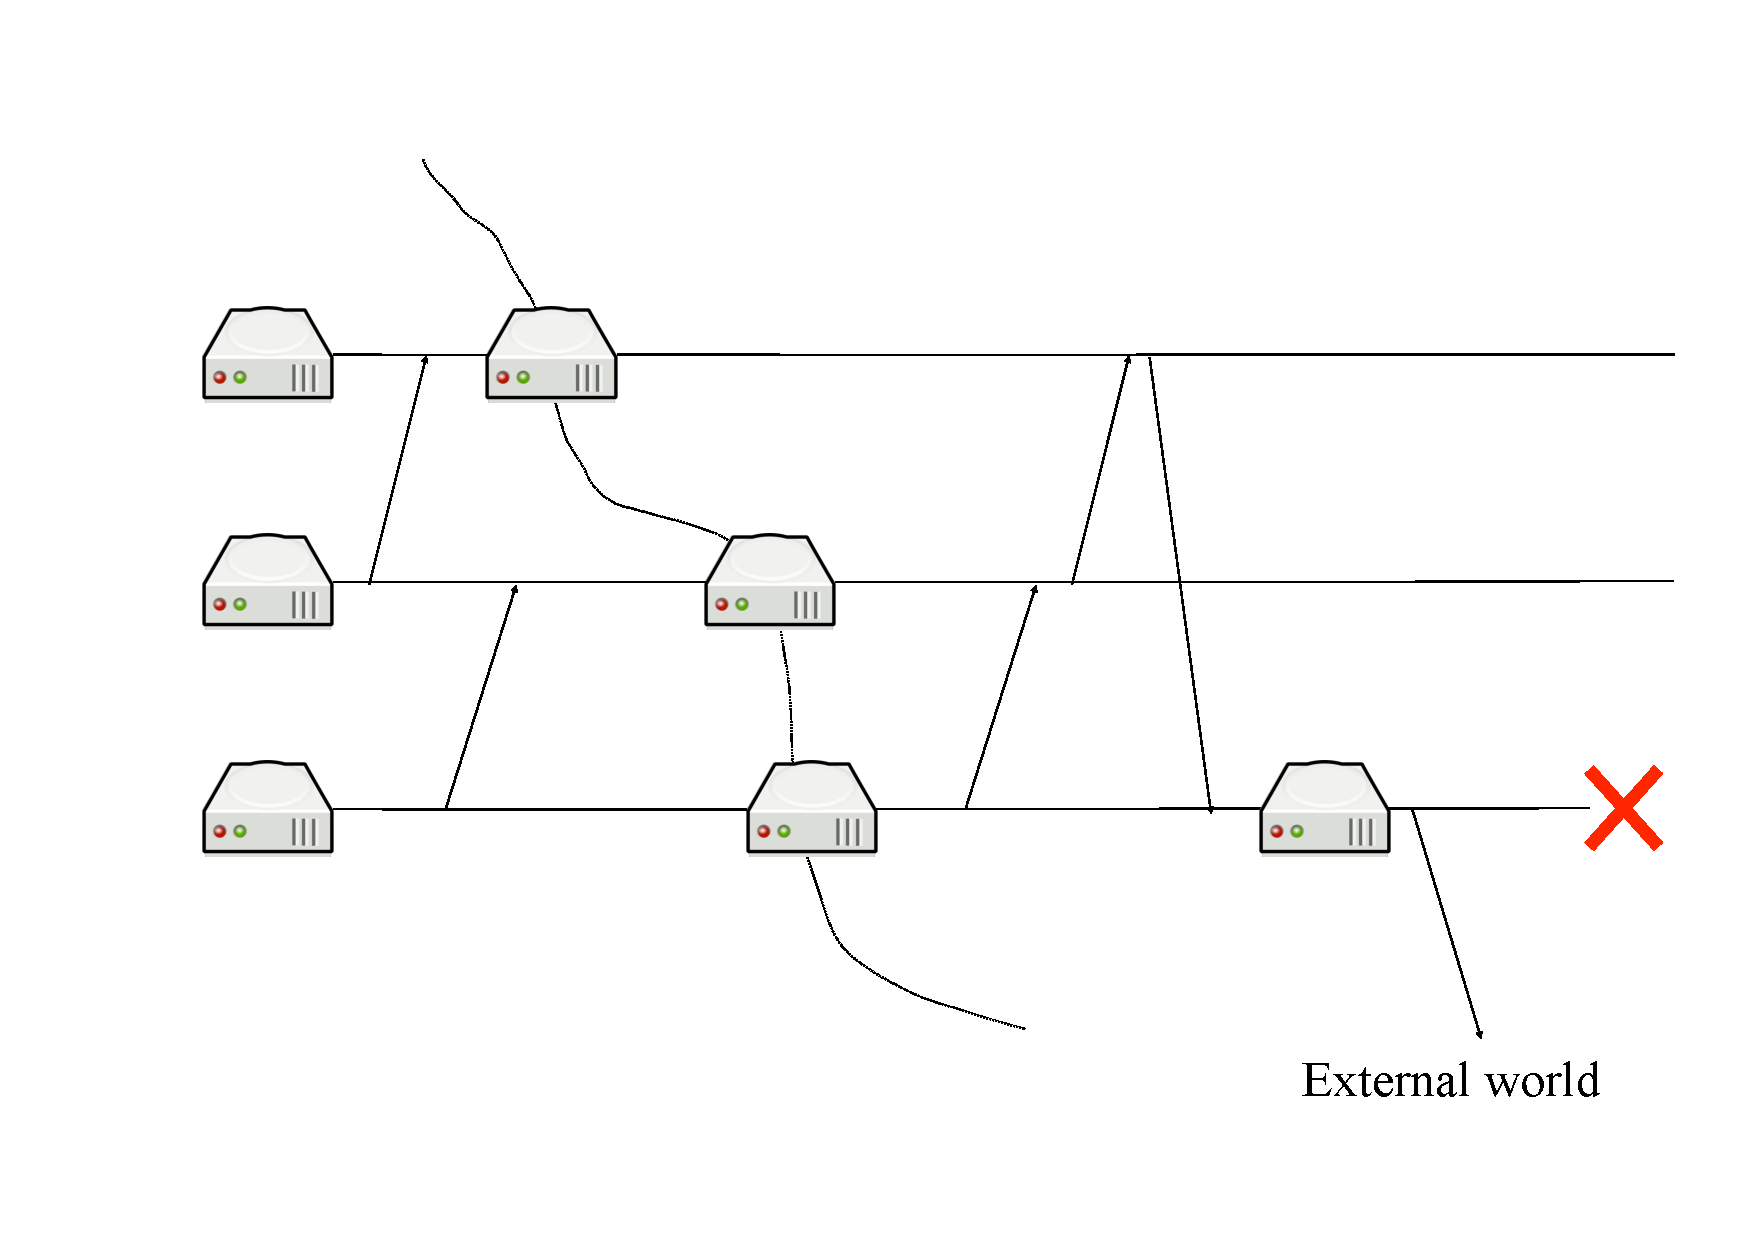
\includegraphics[width=\textwidth,page=1]{output-commit}
\onslide<2|handout:2>
\includegraphics[width=\textwidth,page=2]{output-commit}
\end{overprint}

\end{frame}

%-------------------------------------------------------------------------
\begin{frame}{Garbage collection}
\BI
\item Checkpoints and event logs consume storage resources
\BI
\item Can grow in an unbounded way
\item Subset of the stored information becomes useless
\EI
\item Garbage collection – common approach
\BI
\item Identify the most recent consistent set of checkpoints, which is called the recovery line
\item Discard all information relating to events that occurred before the line
\EI
\item Pragmatic problem – but an important one
\EI
\end{frame}

\section{Algorithms}

%-------------------------------------------------------------------------
\begin{frame}{Rollback-recovery - Taxonomy}
\begin{overprint}
\onslide<1|handout:0>
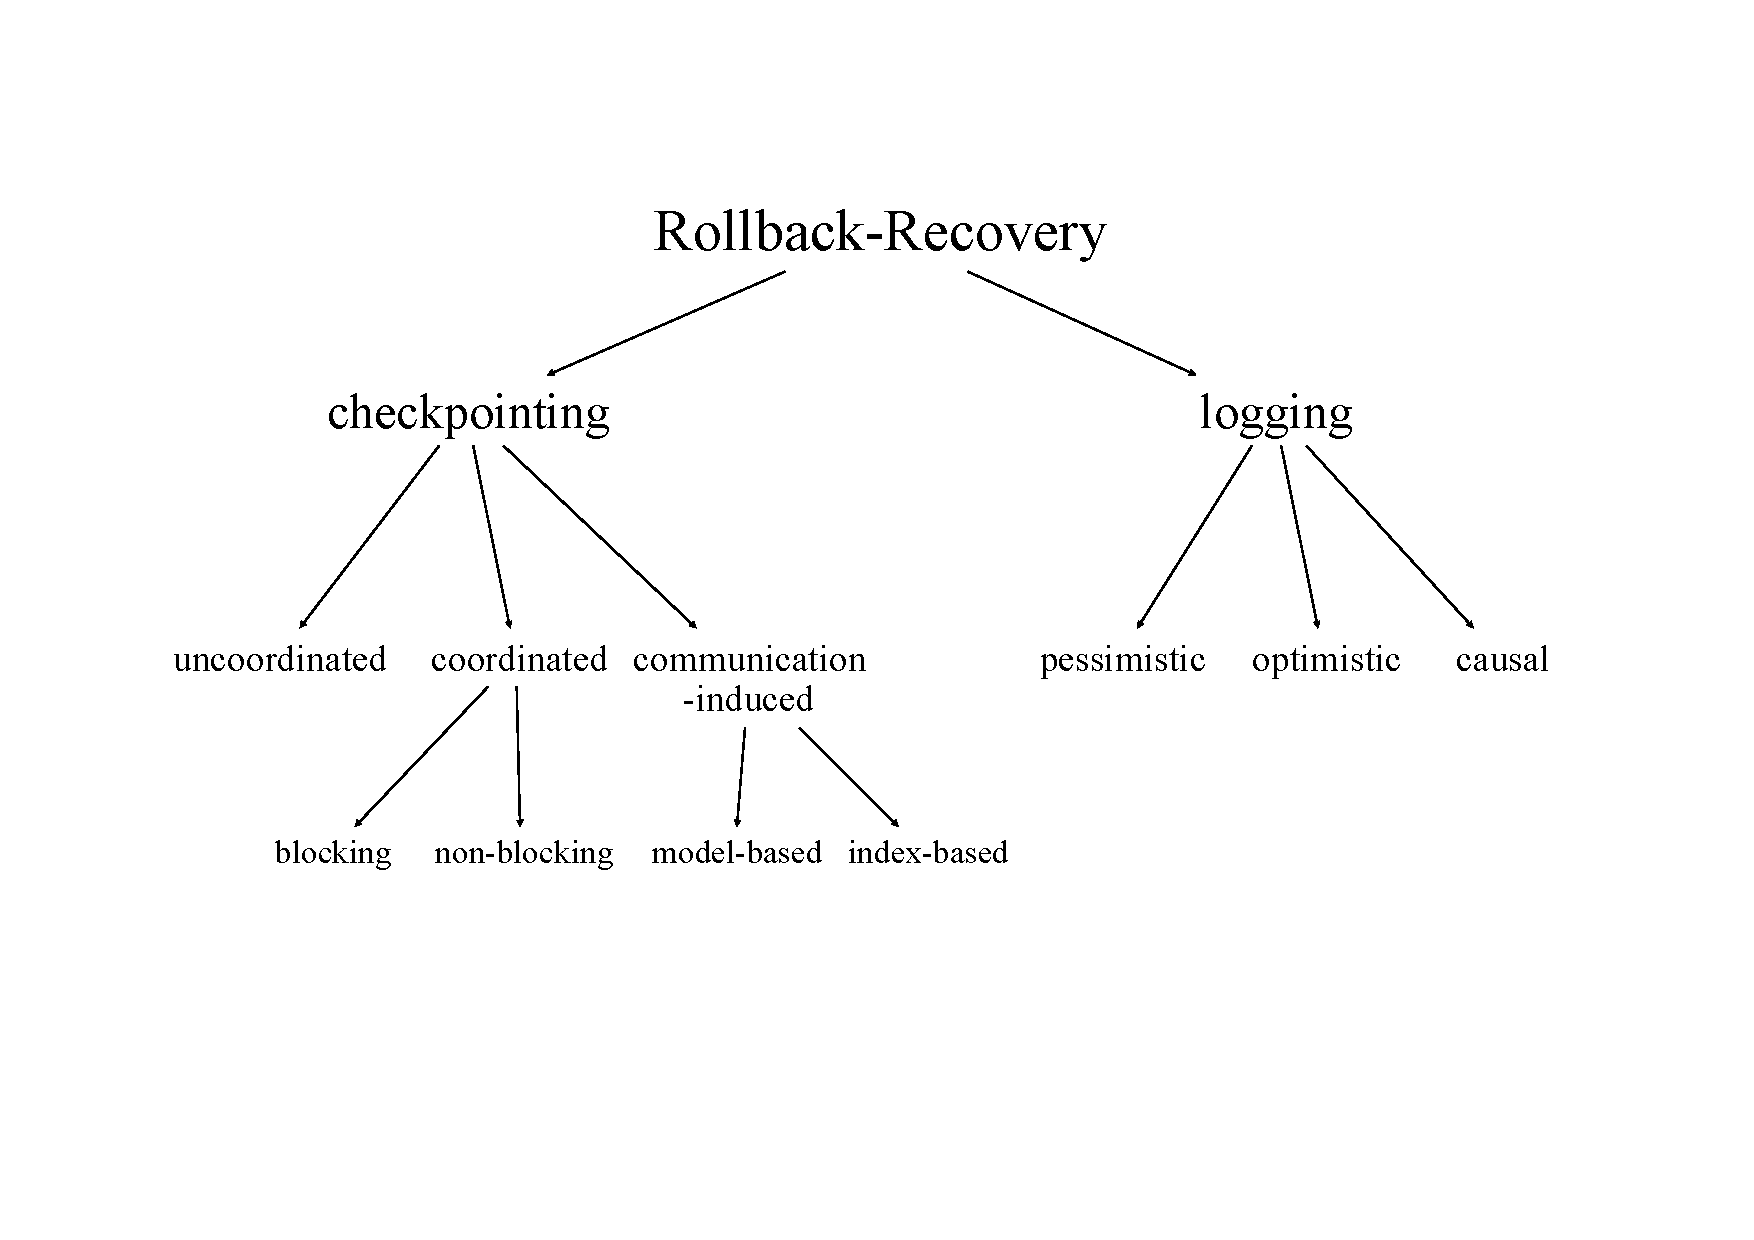
\includegraphics[width=\textwidth,page=1]{taxonomy.pdf}
\onslide<2|handout:1>
\includegraphics[width=\textwidth,page=2]{taxonomy.pdf}
\end{overprint}
\end{frame}

\subsection{Uncoordinated checkpointing}

%-------------------------------------------------------------------------
\begin{frame}{Uncoordinated checkpointing}
	
\BI
\item How it works
\BI
\item Each process autonomously decide when a checkpoint is needed
\EI
\item Advantages
\BI
\item Autonomy – take a checkpoint when it is most convenient
\item e.g., when the amount of information to save is small
\EI
\item Disadvantages
\BI
\item Susceptible to domino effect
\item Can generate useless checkpoints
\item Complicates storage / garbage collection
\item Not suitable for frequent output commits
\item Coordination among all processes to compute recovery lines, thus neglecting autonomy	
\EI
\EI
	
\end{frame}

%-------------------------------------------------------------------------
\begin{frame}{Uncoordinated checkpointing}

\begin{definition}
\BI
\item let $C_{i,x}$ be the $x$-th checkpoint of process $P_i$
\item let $I_{i,x}$ be the interval between checkpoints $C_{i,x-1}$ and $C_{i,x}$
\EI
\end{definition}

\begin{block}{Procedure}
\BI
\item  if $P_i$ sends a message $m$ to $P_j$ during $I_{i,x}$  and $P_j$ receives $m$ during $I_{j,y}$
\BI
\item $P_i$ piggybacks $(i,x)$ on $m$
\item $P_j$ records the dependency from $I_{i,x}$ to $I_{j,y}$ \ldots
\item \ldots which is later stored on stable storage when $P_j$ takes $C_{j,y}$
\EI
\EI
\end{block}

\vspace{-8pt}
\begin{center}
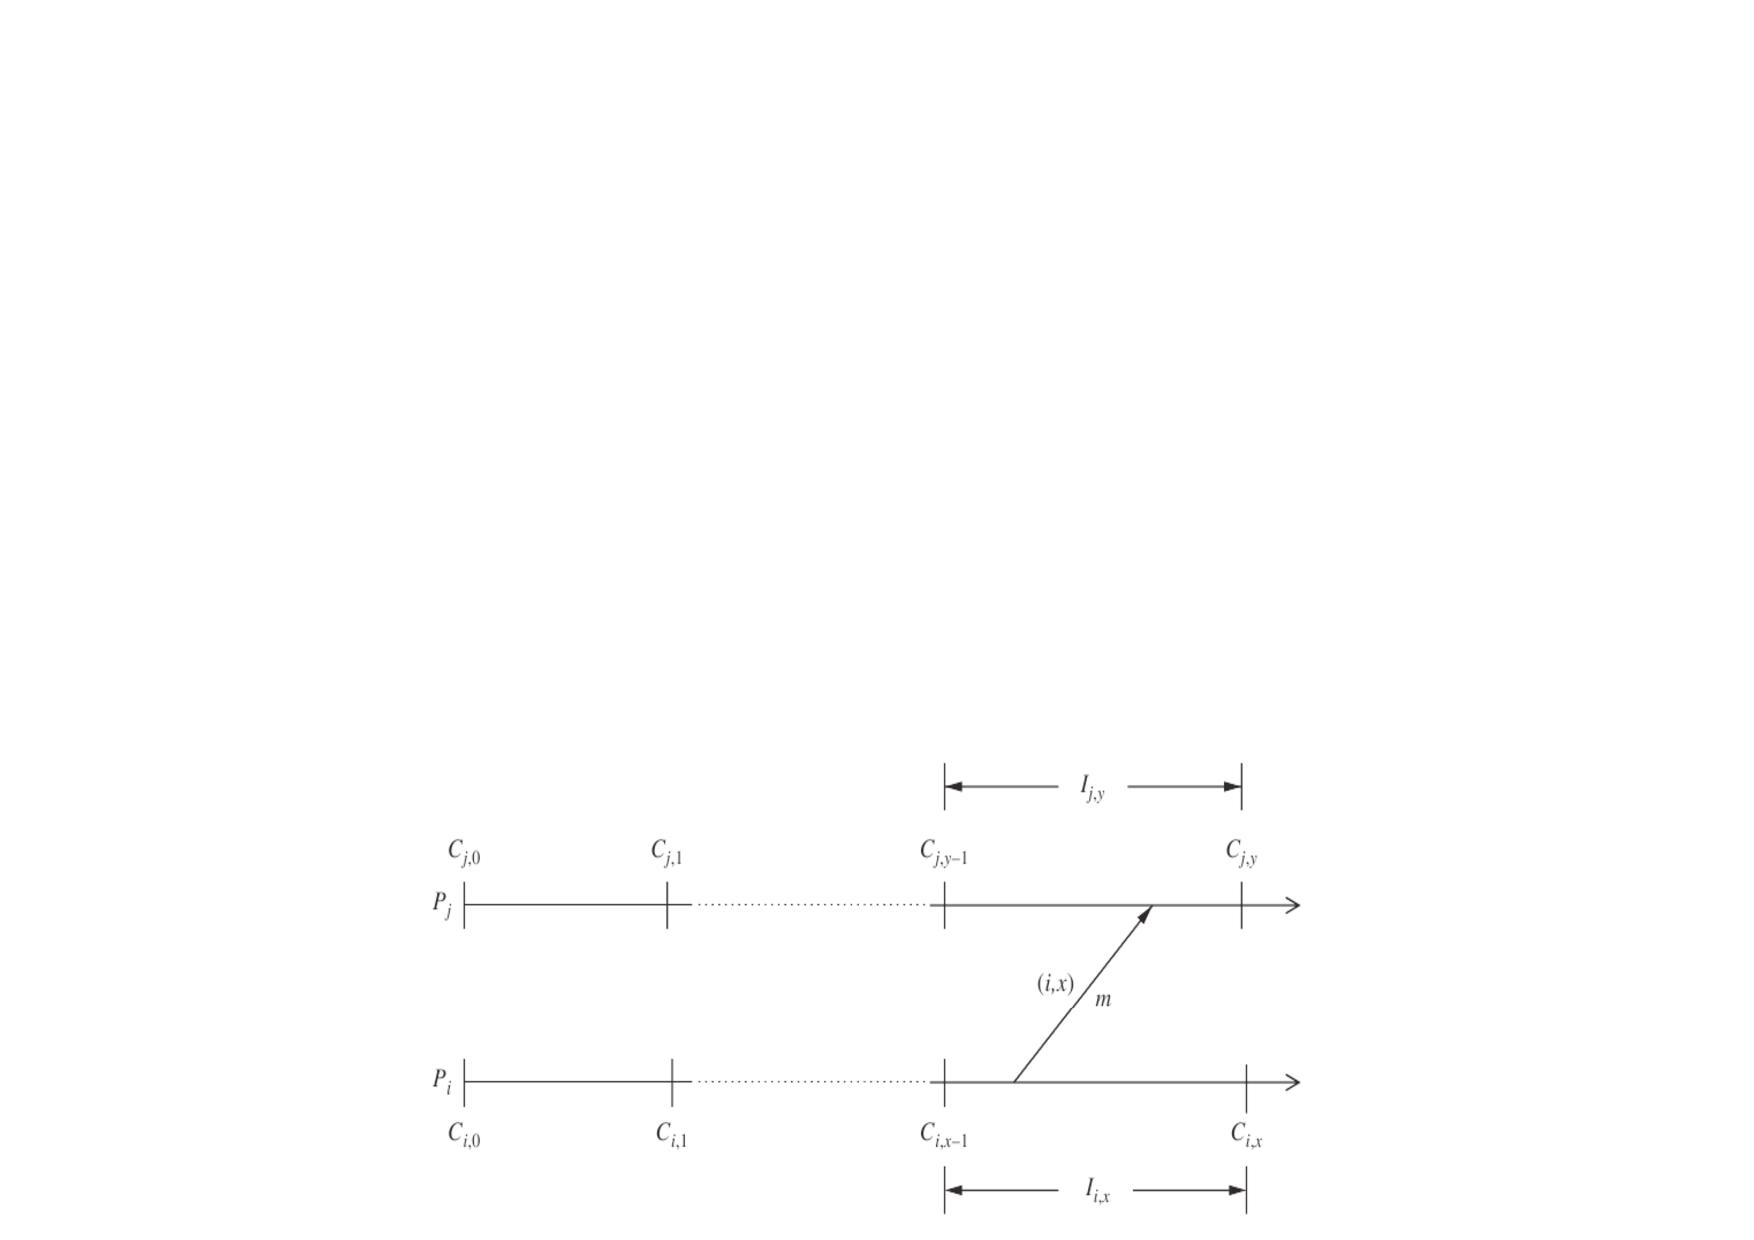
\includegraphics[width=0.5\textwidth]{recovery}
\end{center}

\end{frame}


%-------------------------------------------------------------------------
\begin{frame}{Uncoordinated checkpointing}

\BI	
\item To initiate a recovery
	\BI
	\item Broadcast a dependency request to collect all dependency information maintained at each process
	\item When a process receives this message
		\BI 
		\item it stops its execution
		\item replies with dependencies stored on stable storage and those associated to current interval
		\EI
	\EI
\item The recovering process
	\BI
	\item Computes the recovery line
	\item Sends a rollback request containing the recovery line
	\EI
\item When a process receives the rollback request
	\BI
	\item Resume execution from specified checkpoint
	\EI
\EI
\end{frame}

%-------------------------------------------------------------------------
\begin{frame}{Uncoordinated checkpointing}

\BI
\item \alert{Garbage collection}
	\BI
	\item can be based on periodically computing the recovery line and removing all the checkpoints prior to it
	\EI
\item \alert{Removing "useless checkpoints"}
	\BI
	\item can be done in the same way
	\EI
\item \alert{The big problem}
	\BI
	\item The "domino" effect
	\EI
\EI


\end{frame}

%-------------------------------------------------------------------------
\begin{frame}{The "domino" effect}
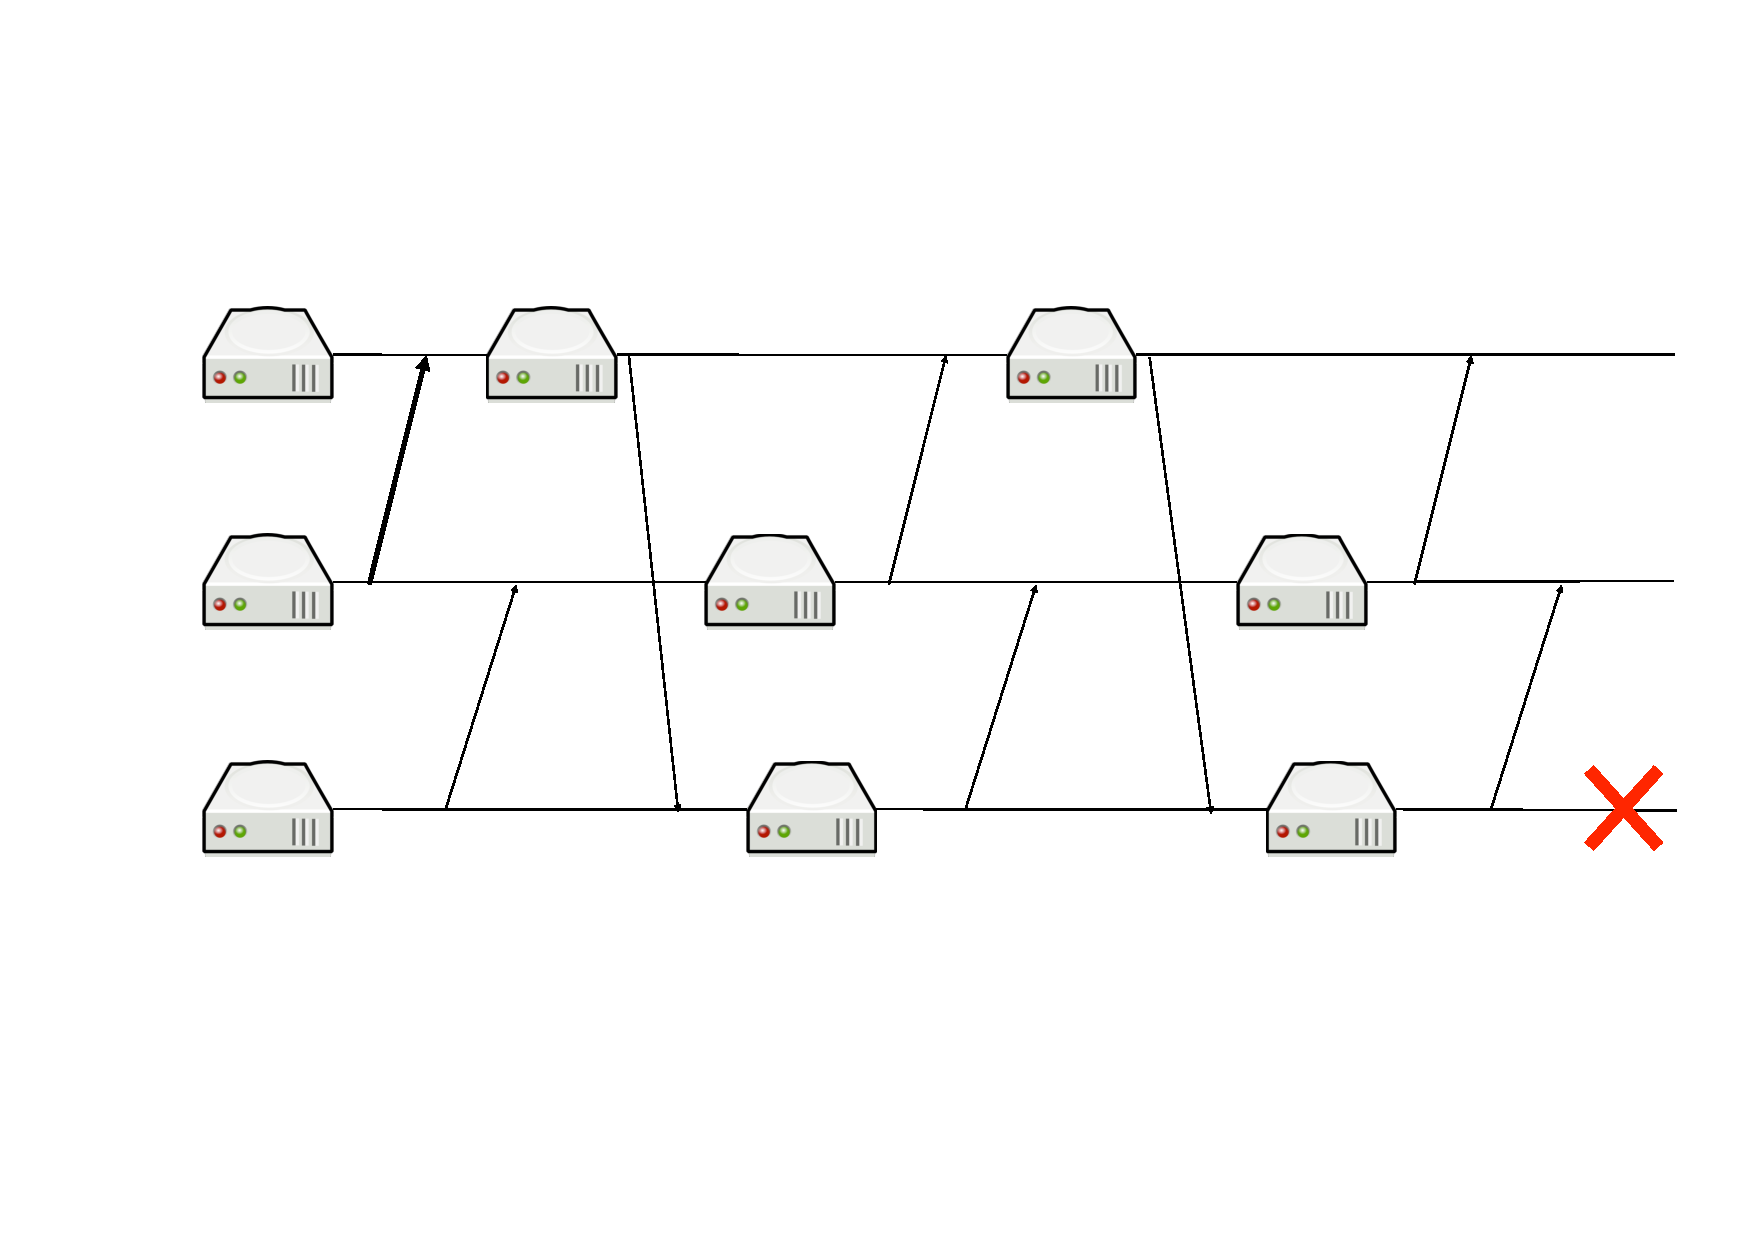
\includegraphics[width=\textwidth]{domino}
\end{frame}

\subsection{Coordinated checkpointing}

%-------------------------------------------------------------------------

\begin{frame}{Coordinated checkpointing}

\begin{definition}
Coordinated checkpointing requires processes to orchestrate their checkpoints in order to form a consistent global state 
\end{definition}

\bigskip
\BI
\item Advantages
	\BI
	\item No domino effect
	\item Each process is required to maintain only one checkpoint (the last)
	\item No computation of recovery line is required
	\EI
\item Disadvantages
	\BI
	\item Large latency in committing output
	\item Two approaches
		\BI
		\item Blocking
		\item Non-blocking
		\EI
	\EI
\EI

\end{frame}

\begin{frame}{Coordinated checkpointing -- blocking}
	
{\def\arraystretch{1.5}
\begin{tabular}{@{\extracolsep{\fill}}  P{0.48\textwidth}  P{0.48\textwidth} }			
\textbf{Coordinator} & \textbf{Processes} \\
\Textbullet sends "take checkpoint" to all & \\
\hfill $\longrightarrow\quad$ & \Textbullet suspend execution \\
& \Textbullet flush all messages \\
& \Textbullet take "tentative" checkpoints \\
& \Textbullet send ack \\
\Textbullet collects ack & $\longleftarrow$\\
\Textbullet sends "commit" message & \\
\hfill $\longrightarrow\quad$ & \Textbullet take "permanent" checkpoints \\
\end{tabular}
}

\end{frame}

\begin{frame}{Coordinated checkpointing --  non-blocking}
\BI
\item Goal – prevent orphan messages (avoid inconsistencies)
\item Does it ring a bell?
\EI

\bigskip
\begin{center}
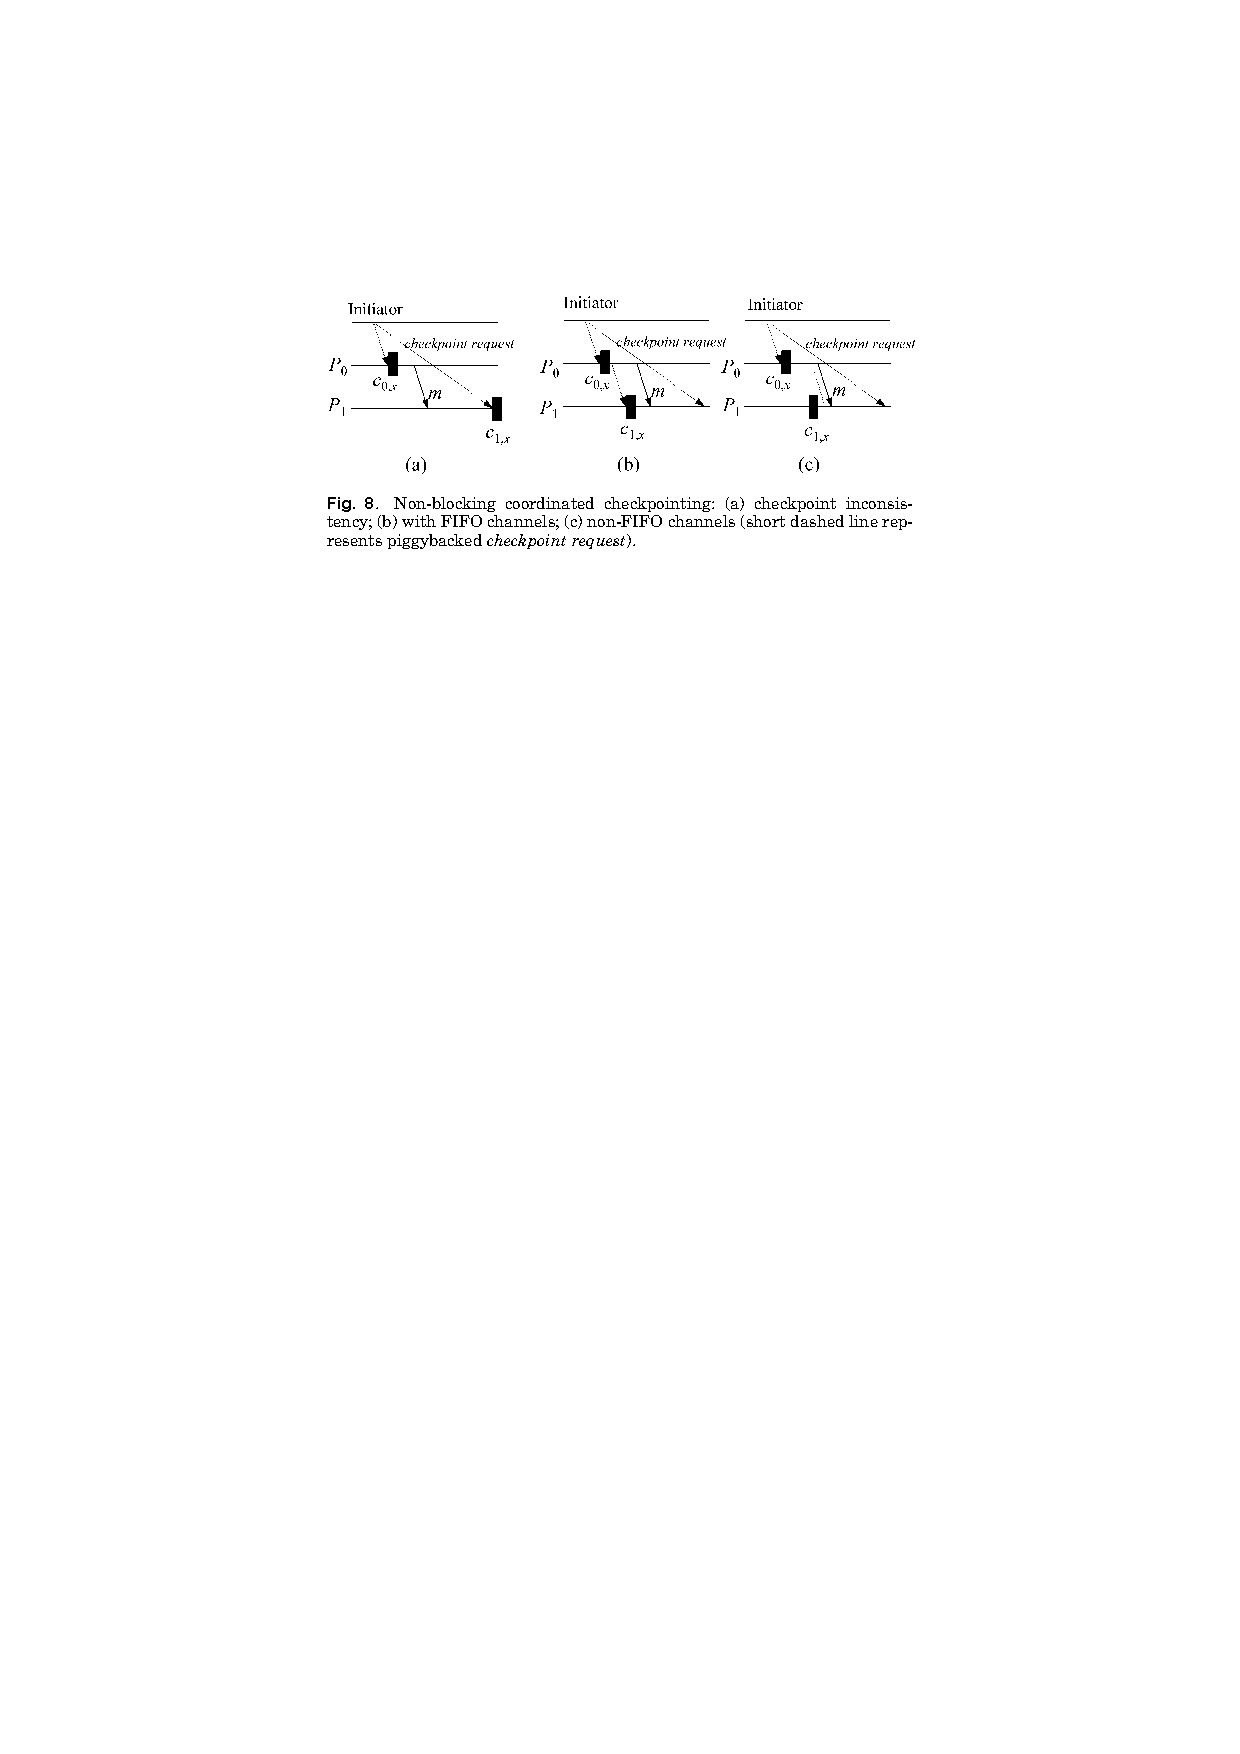
\includegraphics[width=0.9\textwidth]{nonblocking}
\end{center}


\end{frame}


\begin{frame}{Coordinated checkpointing --  non-blocking}
\BI
\item Snapshot protocol (Chandy - Lamport)
\item In-transit messages must be recorded
\EI

\bigskip
\begin{center}
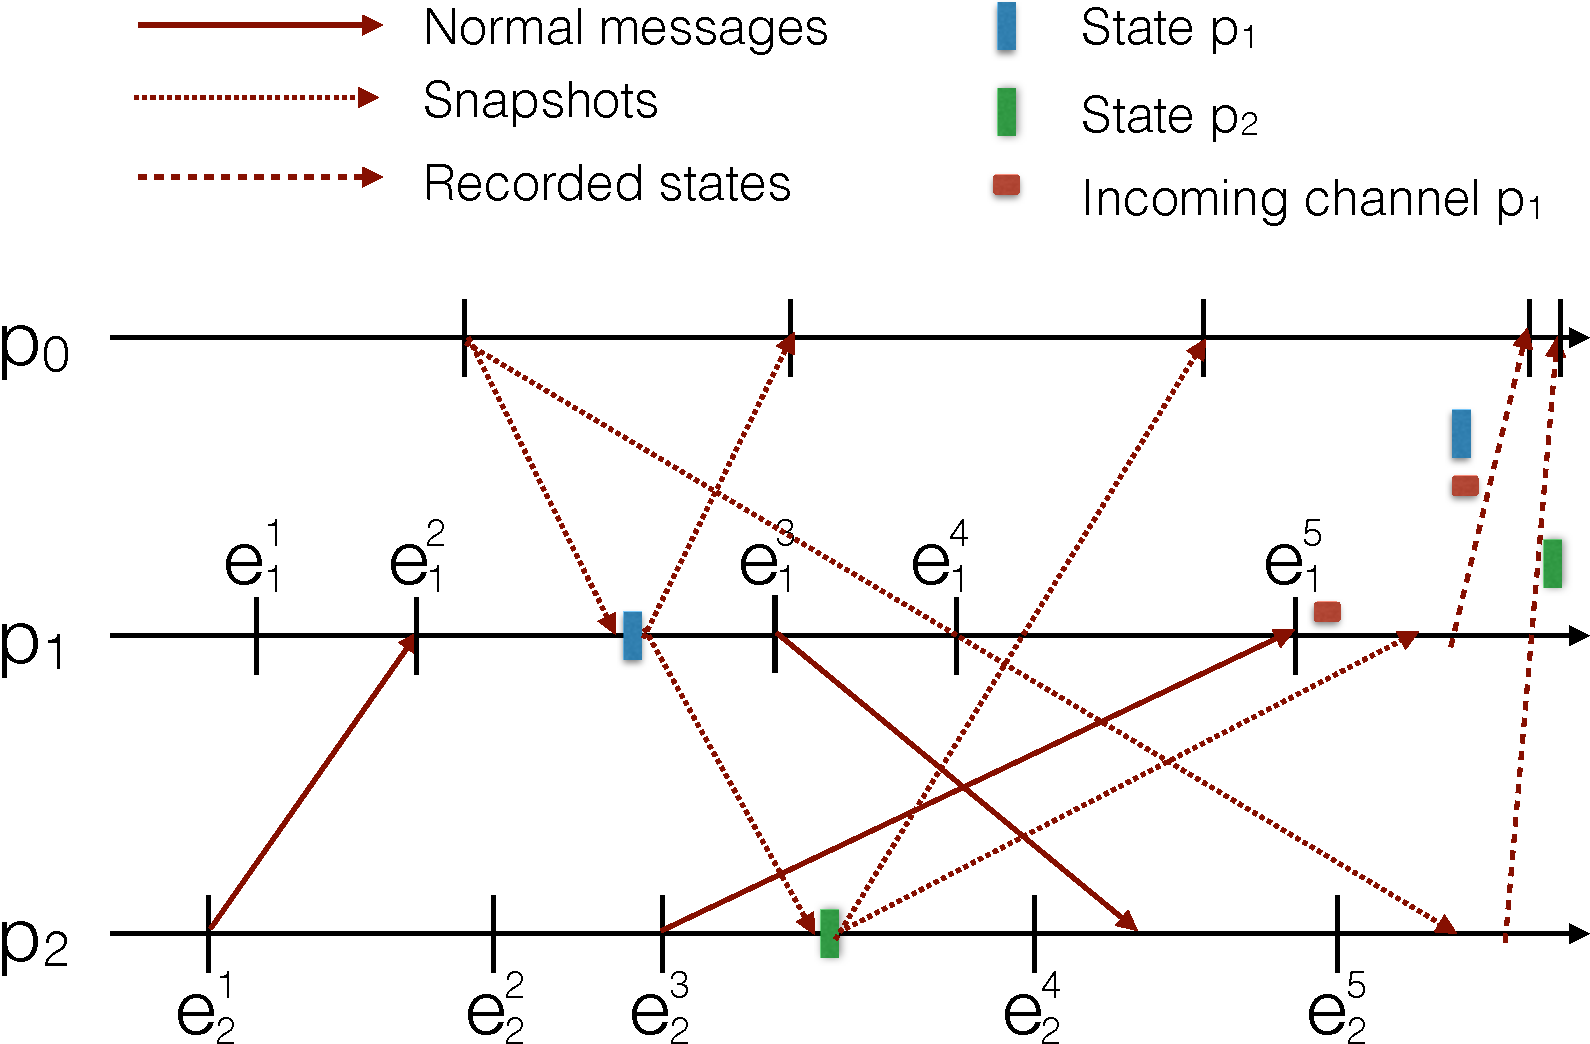
\includegraphics[width=0.7\textwidth]{figs/03/diagram9}
\end{center}

\end{frame}

\begin{frame}{Coordinated checkpointing}
\BI
\item Minimal checkpointing coordination
	\BI
	\item Coordinated checkpointing requires all processes to participate
	\item Scalability problem
	\EI
\item Kuo and Toueg, 1987
	\BI
	\item Only processes that communicated (directly or indirectly) with the coordinator need to take a checkpoint
	\item Can be identified through recursive message sending
	\EI
\EI
\end{frame}

\subsection{Communication-induced checkpointing}

\begin{frame}{Communication-induced checkpointing (CIC)}
\BI
\item How CIC works?
	\BI
	\item No special coordination messages
	\item Information piggybacked on application messages
	\EI
\item Informally
	\BI
	\item Check whether past communication and checkpoints pattern can lead to the creation of a useless checkpoint
	\item A forced checkpoint is taken to break these patterns
	\item Elegant theory based on \alert{Z-paths} and \alert{Z-cycles}	
	\EI
\EI
\end{frame}

\begin{frame}{Z-Paths}

\begin{overprint}
\onslide<1|handout:1>
\begin{block}{Definitions}
\BI 
\item Let $\rightarrow$ denote the happen-before relation of Lamport
\item Let $C_{i,x}$ denote the $x$-th checkpoint of process $P_i$
\item Let $I_{i,x}$ denote the interval between $C_{i-1,x}$ and $C_{i,x}$
\EI
\end{block}
\onslide<2|handout:2>
\begin{center}
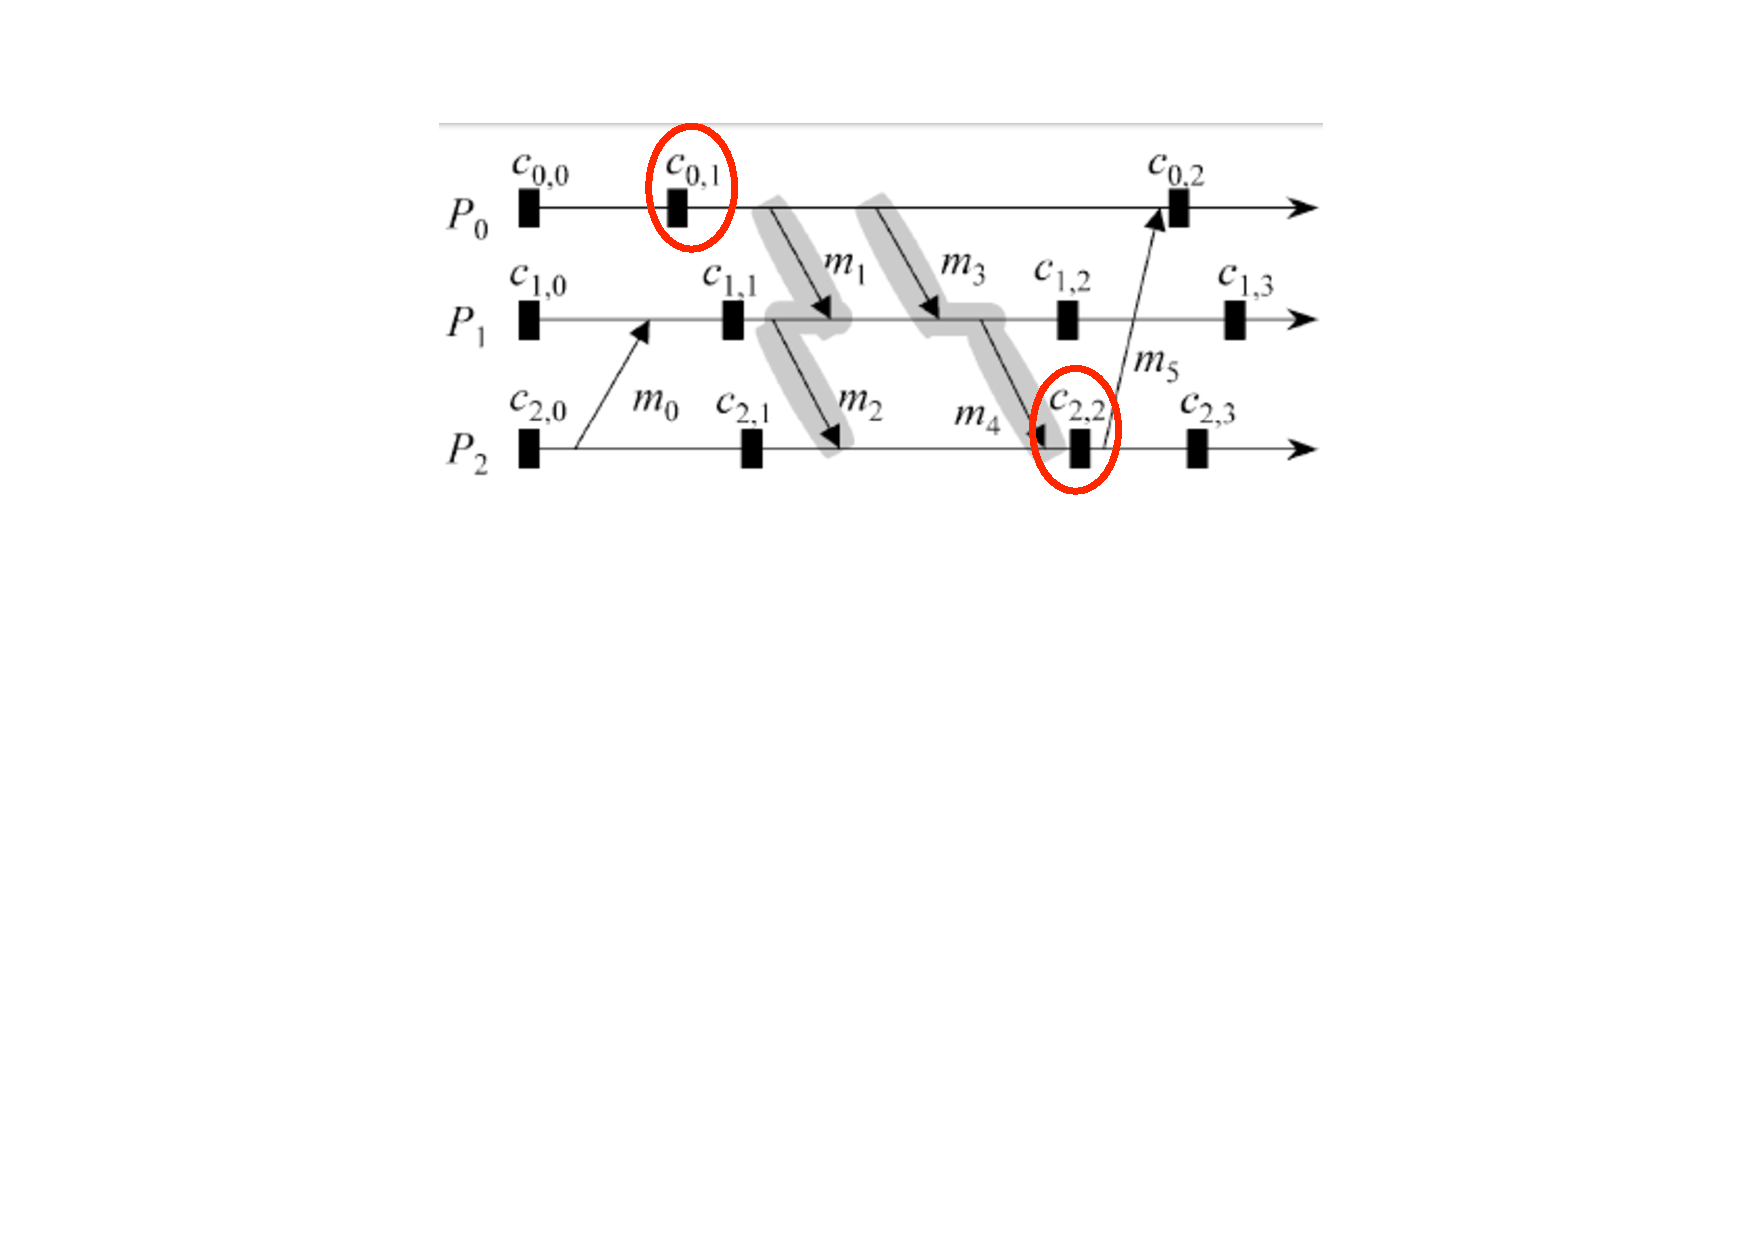
\includegraphics[width=0.5\textwidth]{zpath1}
\end{center}
\end{overprint}

\vspace{-66pt}
\begin{block}{Z-path}
Given two checkpoints $C_{i,x}$ and $C_{j,y}$, a \alert{Z-path} exists between them if 
and only if one of the following conditions holds:
\BI
\item $x<y$ and $i=j$, or
\item there exists a sequence $[m_0, m_1, ..., m_n]$, $n>0$ such that
	\BI
	\item $C_{i,x} \rightarrow \send_i(m_0)$
	\item for all $b < n$, either $\receive_k(m_b)$ and $\send_k(m_{b+1})$ belongs 
	to the same checkpoint interval, or $\receive_k(m_b) \rightarrow \send_k(m_{b+1})$
	\item $\receive_j(m_n) \rightarrow C_{j,y}$
	\EI
\EI
\end{block}

\end{frame}

\begin{frame}{Z-cycle}
\begin{center}
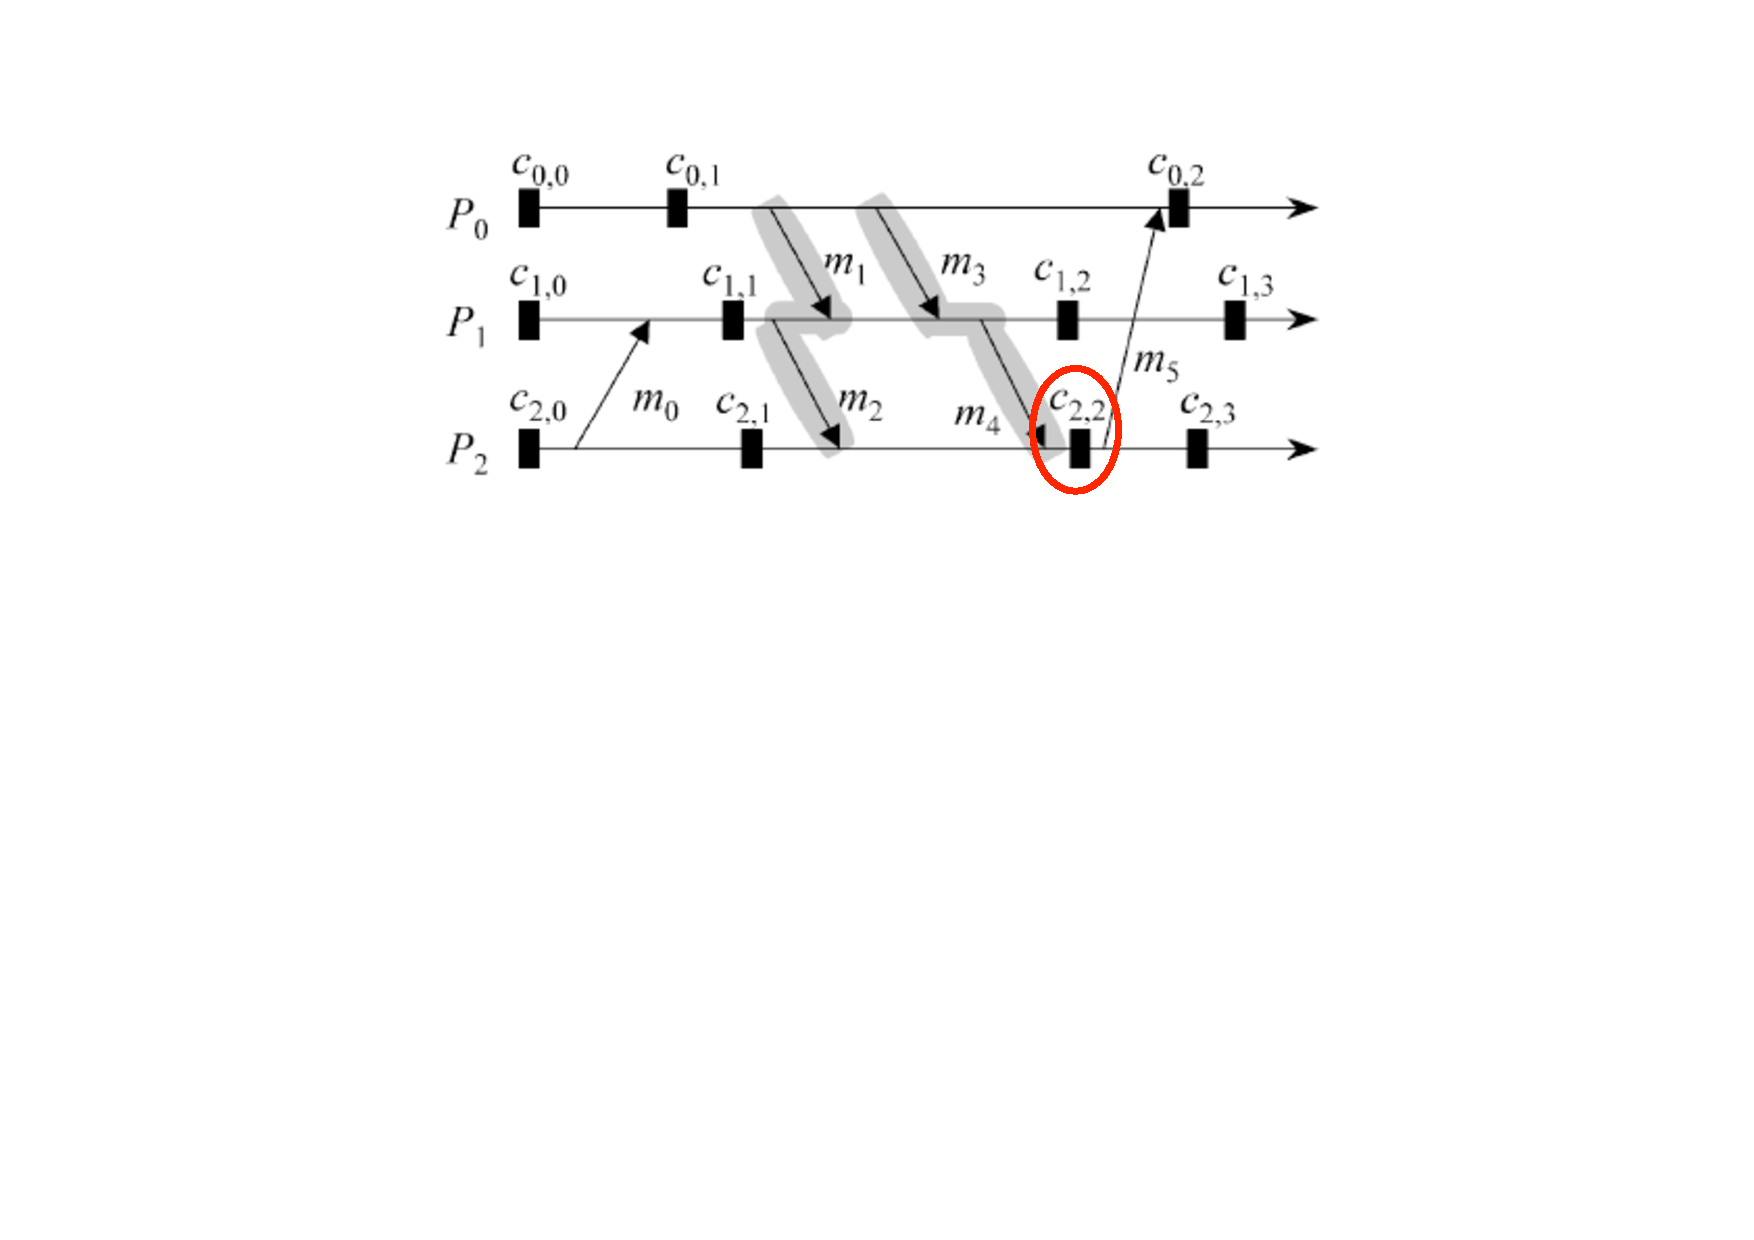
\includegraphics[width=0.5\textwidth]{zpath2}
\end{center}

\begin{block}{Z-Cycles}
\BI
\item A \alert{Z-cycle} is a Z-path that begins and ends with the same checkpoint
\item Example: $[m_5, m_3, m_4]$
\item It can be proved (Netzer and Xu, 1995) that a checkpoint is useless if and 
only if is part of a Z cycle
\item  If we avoid Z-cycles $\rightarrow$ we avoid useless checkpoints
\EI
\end{block}

\end{frame}

\begin{frame}{Communication-induced checkpointing}
\BI
\item Model-based checkpointing
	\BI
	\item A model is set up to detect the possibility that Z-paths occurs 
	\item Each process can locally decide whether a forced checkpoint is required
	\EI
\item Problems
	\BI
	\item Forced checkpoints are un-coordinated
	\item Several additional checkpoints can be forced by distinct processes
	\EI
\EI
\end{frame}

\section{Log-based rollback recovery}

%-------------------------------------------------------------------------
\begin{frame}{Rollback-recovery - Taxonomy}
\begin{overprint}
\onslide<1|handout:0>
\includegraphics[width=\textwidth,page=2]{taxonomy.pdf}
\onslide<2|handout:1>
\includegraphics[width=\textwidth,page=3]{taxonomy.pdf}
\end{overprint}
\end{frame}

%-------------------------------------------------------------------------
\begin{frame}{Log-based rollback recovery}

\BI
\item \alert{Message Logging}
	\BI
	\item Can avoid domino effect
	\item Works with coordinated checkpoint
	\item Works with uncoordinated checkpoint
	\item Can reduce cost of output commit
	\item \alert{More difficult to implement}
	\EI
\item Not limited to "messages" though; the name comes from historical reasons
\EI
\end{frame}

%-------------------------------------------------------------------------
\begin{frame}{Log-based rollback recovery}
	
\begin{definition}[Deterministic state intervals]
The execution of an algorithm started by a non-deterministic event
	\BI
	\item Message receipt
	\item Internal events
	\EI
Note: message sending is not non-deterministic
\end{definition}

\bigskip
Assumption:
	\BI
	\item All non-deterministic events can be identified and their corresponding determinant can be logged to stable storage
	\EI
\end{frame}
%-------------------------------------------------------------------------
\begin{frame}{Log-based rollback-recovery}
\BIL
\item \alert{How it works}
	\BI
	\item Each process logs on stable storage the determinants of all non-deterministic events
	\item Additionally, checkpoints are taken to reduce the extent of rollback during recovery
	\EI
\item \alert{In case of recovery}
	\BI
	\item Checkpoints are used to restore state
	\item Nondeterministic events are replayed precisely as they occurred
	\item Recovery works up to the first non-deterministic event whose determinant is not logged
	\EI
\item What are \alert{determinants}, exactly?
\EIL
\end{frame}
%-------------------------------------------------------------------------
\begin{frame}{Orphan process}
\begin{definition}[Orphan process]
A process $p$ becomes an orphan when $p$ does not fail and $p$'s state depends on the execution of a nondeterministic event e whose determinant cannot be recovered
\BI
\item from stable storage
\item from the volatile memory of a surviving process
\EI
\end{definition}

\bigskip
The management of the orphan process problem may have effects on:
\BI
\item failure-free performance overhead
\item latency of output commit
\item garbage collection
\item recovery mechanism	
\EI

\end{frame}
%-------------------------------------------------------------------------
\begin{frame}[shrink=5]{Logging "flavors"}
	
\begin{block}{Pessimistic}
\BI
\item Orphans never created
\item Simple recovery, garbage collection and output commit
\item High failure-free overhead
\EI
\end{block}
\begin{block}{Optimistic}
\BI
\item Allow orphans to be created
\item Reduce failure overhead
\item Orphans complicate recovery, garbage collection, output commit
\EI
\end{block}
\begin{block}{Causal}
\BI
\item Tries to combine the best of pessimistic, optimistic
	\BI 
	\item Low performance overhead
	\item Fast output commit
	\EI
\item But still complicate recovery, garbage collection
\EI
\end{block}
\end{frame}
%-------------------------------------------------------------------------
\begin{frame}{Specification}
	
Let $e$ be a non-deterministic event executed by $p$

\medskip
\begin{block}{$\mathit{depend}(e)$}
The set of processes that are affected by $e$ i.e, $p$ plus any process whose state depends on $e$ according to Lamport's happened-before
\end{block}
\begin{block}{$\mathit{log}(e)$}
The set of processes that have logged a copy of $e$ in their volatile memory
\end{block}
\begin{block}{$\mathit{stable}(e)$}
A predicate that is true if $e$'s determinant is logged on stable storage
\end{block}
\end{frame}
%-------------------------------------------------------------------------
\begin{frame}{Specification}
	
\begin{block}{Always-no-orphan}
\BI
\item $\NOT\ \mathit{stable}(e) \Rightarrow \mathit{depend}(e) \subseteq \mathit{log}(e)$
\item if a process depends on a event $e$, either $e$ is on stable storage, or the process has a copy of the determinant of event $e$
\item otherwise, it is orphan
\EI
\end{block}

% \bigskip
% Compare it with "eventually-no-orphan"
% \BI
% \item Processes may become orphan but eventually they recover to a non-orphan state
% \EI

\subsection{Pessimistic logging}
	
\end{frame}
%-------------------------------------------------------------------------
\begin{frame}{Pessimistic logging}
\begin{block}{Pessimistic approach}
\BI
\item Failures can happen – at any time!
\item (In reality, failures are rare)
\EI
\end{block}

\medskip
How it works:
\BI
\item Each nondeterministic event is logged on stable storage before it can affect the computation 
\item Synchronous logging: $\NOT\ \mathit{stable}(e) \Rightarrow \mathit{depend}(e) = \emptyset$
\item It is a stronger version of Always-no-orphan
\item This property stipulates that if an event has not been logged on stable storage, then no process can depend on it.
\EI

\end{frame}

\begin{frame}{Pessimistic logging}
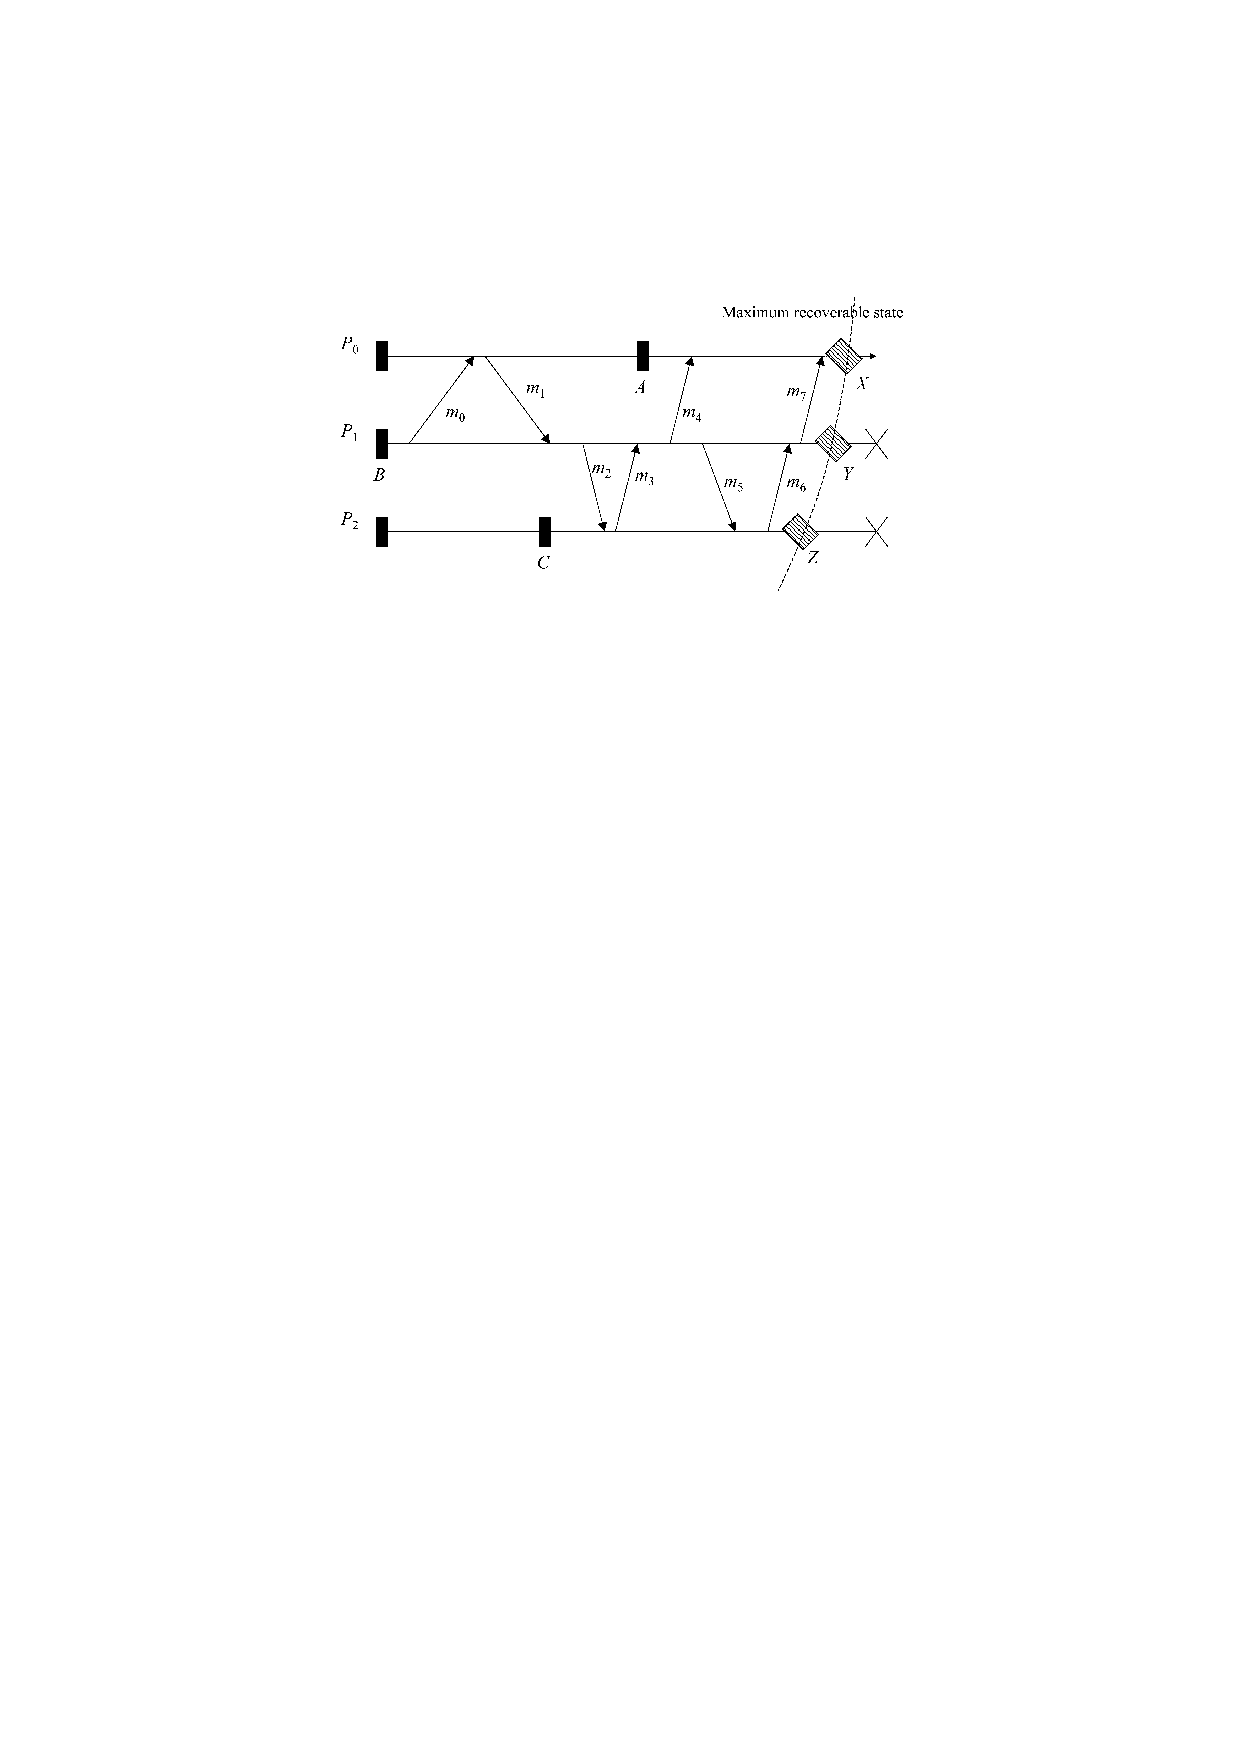
\includegraphics[width=\textwidth]{pessimistic}
\end{frame}

\begin{frame}{Pessimistic logging}
\BIL
\item \alert{Advantages}
	\BI
	\item Interaction with OWP without running a special protocol
	\item Process restart from their most recent checkpoint upon a failure
	\BI
		\item limits the amount of computation that must be replayed
		\item frequency of checkpoints $\rightarrow$ trade-off overhead/protection
	\EI
	\item Recovery is simple
	\BI
		\item The effects of a failure are confined to the processes that fail
		\item Processes never become orphans
	\EI
	\item Garbage collection is simple
	\BI
		\item Collect everything before last checkpoint
	\EI
	\EI
\item \alert{Disadvantages}
	\BI
	\item Performance penalty for synchronous logging
	\EI
\EIL
\end{frame}

\subsection{Optimistic logging}

\begin{frame}{Optimistic logging}
	
\begin{block}{Optimistic approach}
\BI
\item Failures are rare
\item They do not occur before determinant is logged to stable storage
\EI
\end{block}

\medskip
\BIL
\item How it works:
	\BI
	\item Determinants are logged to volatile memory
	\item Periodically flushed to stable storage
	\item No blocking is necessary
	\EI
\item Problem: if a process fails before determinant is written to stable storage,
determinants will be lost
	\BI
	\item other processes may become orphans
	\item always-no-orphans is not guaranteed
	\EI
\EIL

\end{frame}

\begin{frame}{Optimistic logging}
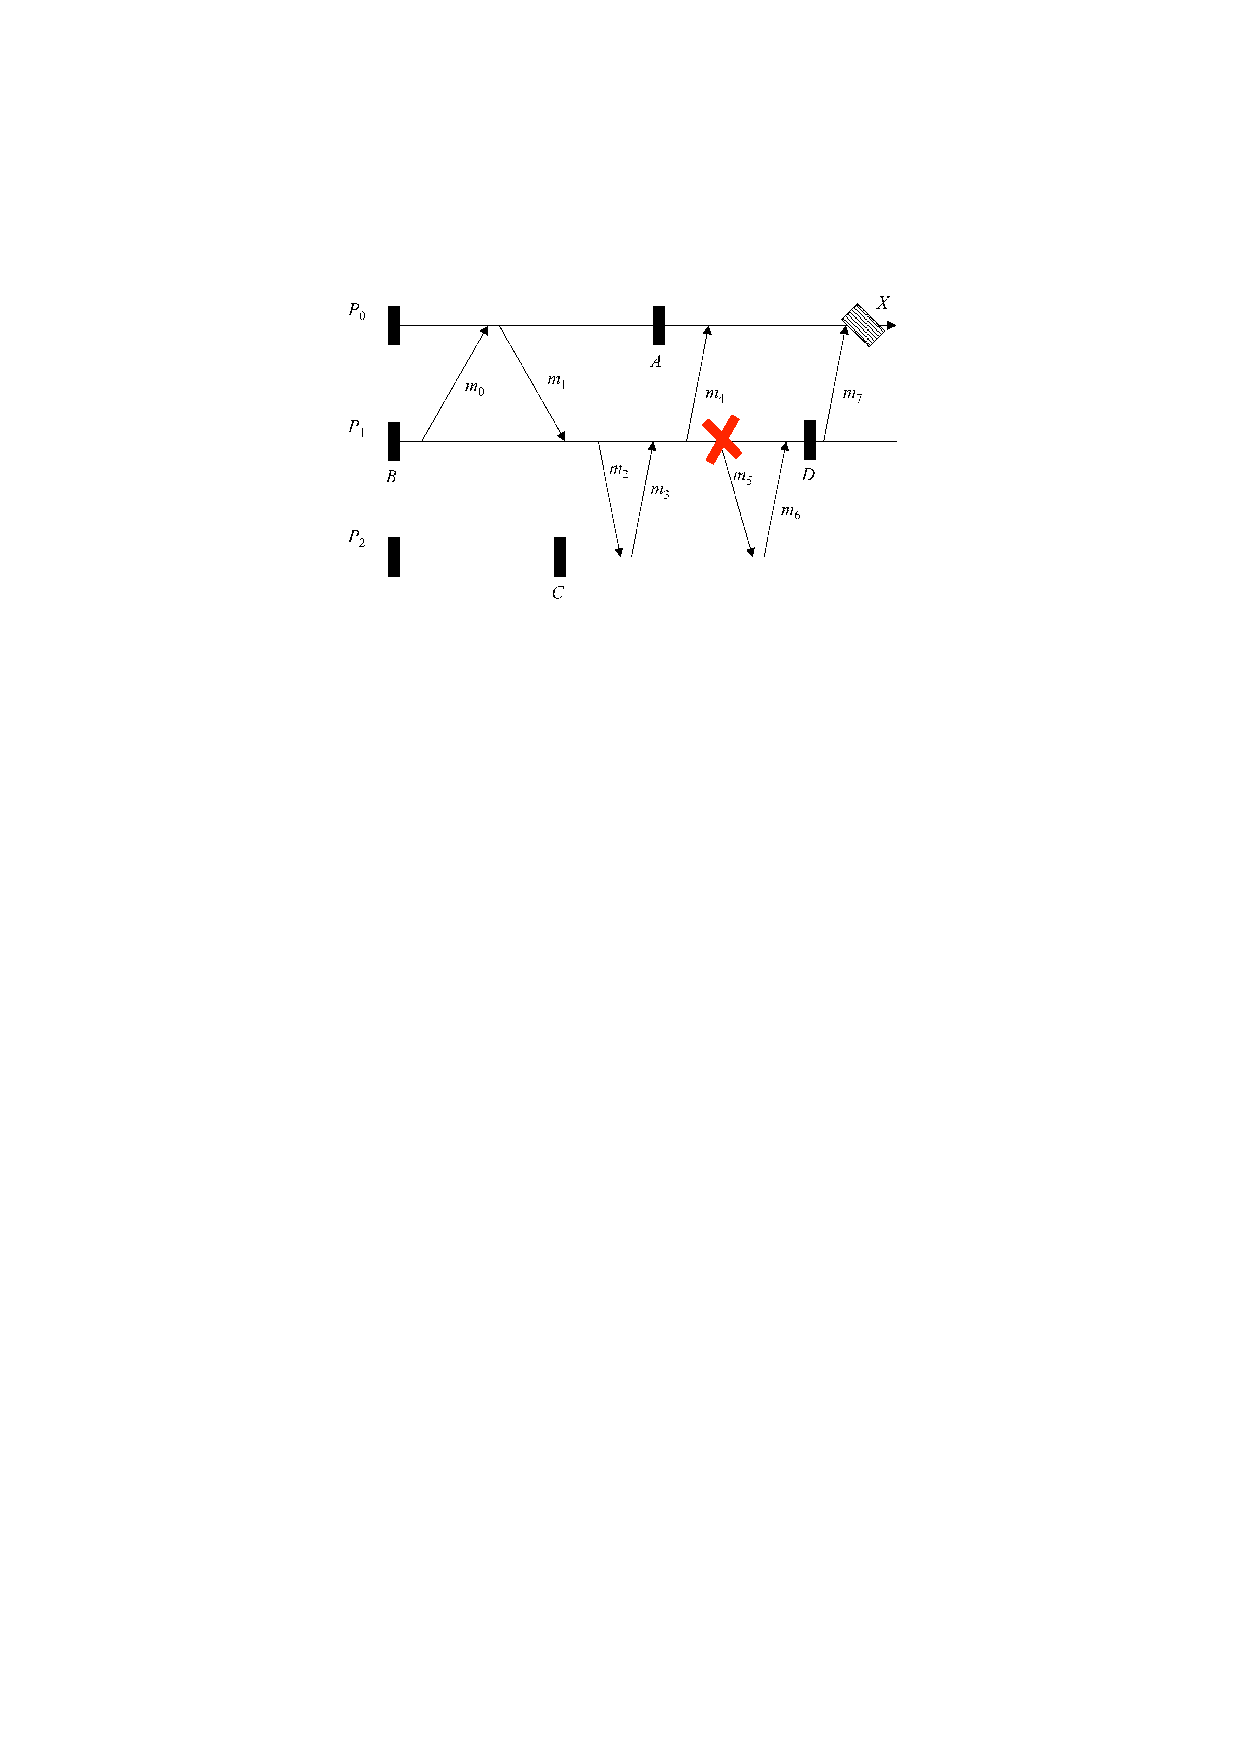
\includegraphics[width=\textwidth]{optimistic}
\end{frame}

\begin{frame}{Optimistic logging}
\BI
\item Problems
\BI
	\item Garbage collection is complex
	\item Recovery is complex
	\item Output commit requires global coordination
\EI
\EI
\end{frame}

\subsection{Causal logging}

\begin{frame}{Causal logging}
\BIL
\item Advantages of optimistic logging
	\BI
	\item Logging is performed asynchronously
	\item (Except for output commit)
	\EI
\item Advantages of pessimistic logging
	\BI
	\item Each process can independently perform output commit
	\item Always-no-orphans is satisfied
	\EI
\item How it works
	\BI
	\item The determinant of each event that causally precedes the state of a process is either stable or available locally to that process
	\item Determinants of causally-preceding events are piggy-backed on messages
	\EI
\EIL
\end{frame}


\begin{frame}
\begin{center}
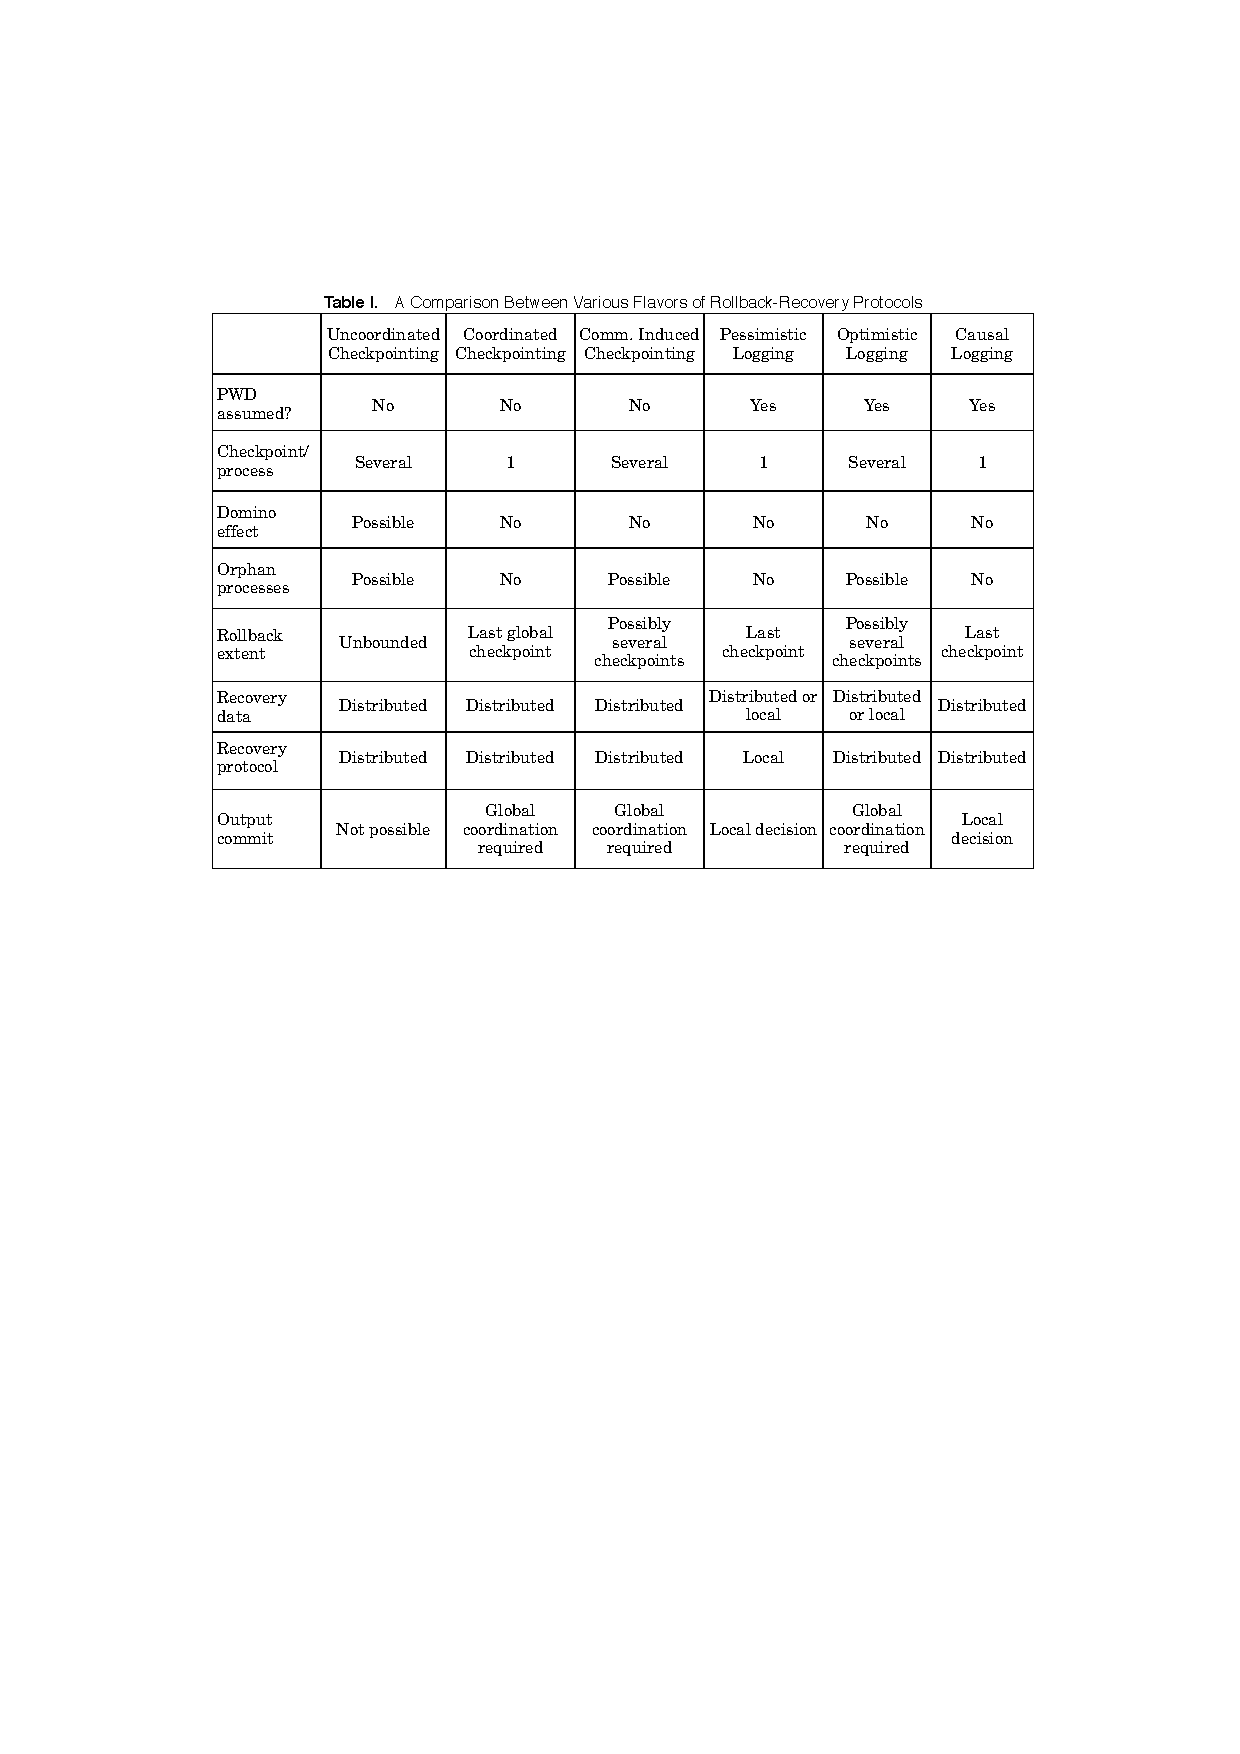
\includegraphics[width=0.93\textwidth]{table}
\end{center}
\end{frame}

%-------------------------------------------------------------------------
\begin{RMFrame}

\BI
\item \bibentry{alvisi-rr}
\EI

\end{RMFrame}

\end{document}